%!TEX root = thesis.tex

\newcommand{\inp}[1]{\input{../out/#1}}
\newcommand{\characteristic}[2]{\inp{#1/characteristics/#2}}
\newcommand{\descriptive}[2]{\inp{#1/descriptive/#2}}
\newcommand{\test}[3]{\inp{#1/test/#2/#3}}
\newcommand{\normaldistr}{$\mathcal{N}(\descriptive{original}{mean}, \descriptive{original}{variance})$}

\newpage

\chapter{Анализ временного ряда в пакете R}

\section{Детерминированный подход} % (fold)
\label{sec:determenistic}

\subsection{Описательные статистики и первичный анализ данных} % (fold)
\label{sec:basis}

В качестве исходных данных примем выборку из полученной от учебно-научного центра базы данных, путём отбора наблюдений в июле месяце за период с 1975 по 2012 год. Выборка представлена в приложении \ref{c:source_data} в таблице \ref{table:source}. Графически исходные данные представлены на рисунке \ref{img:input}.

\begin{figure}[ht]
	\center{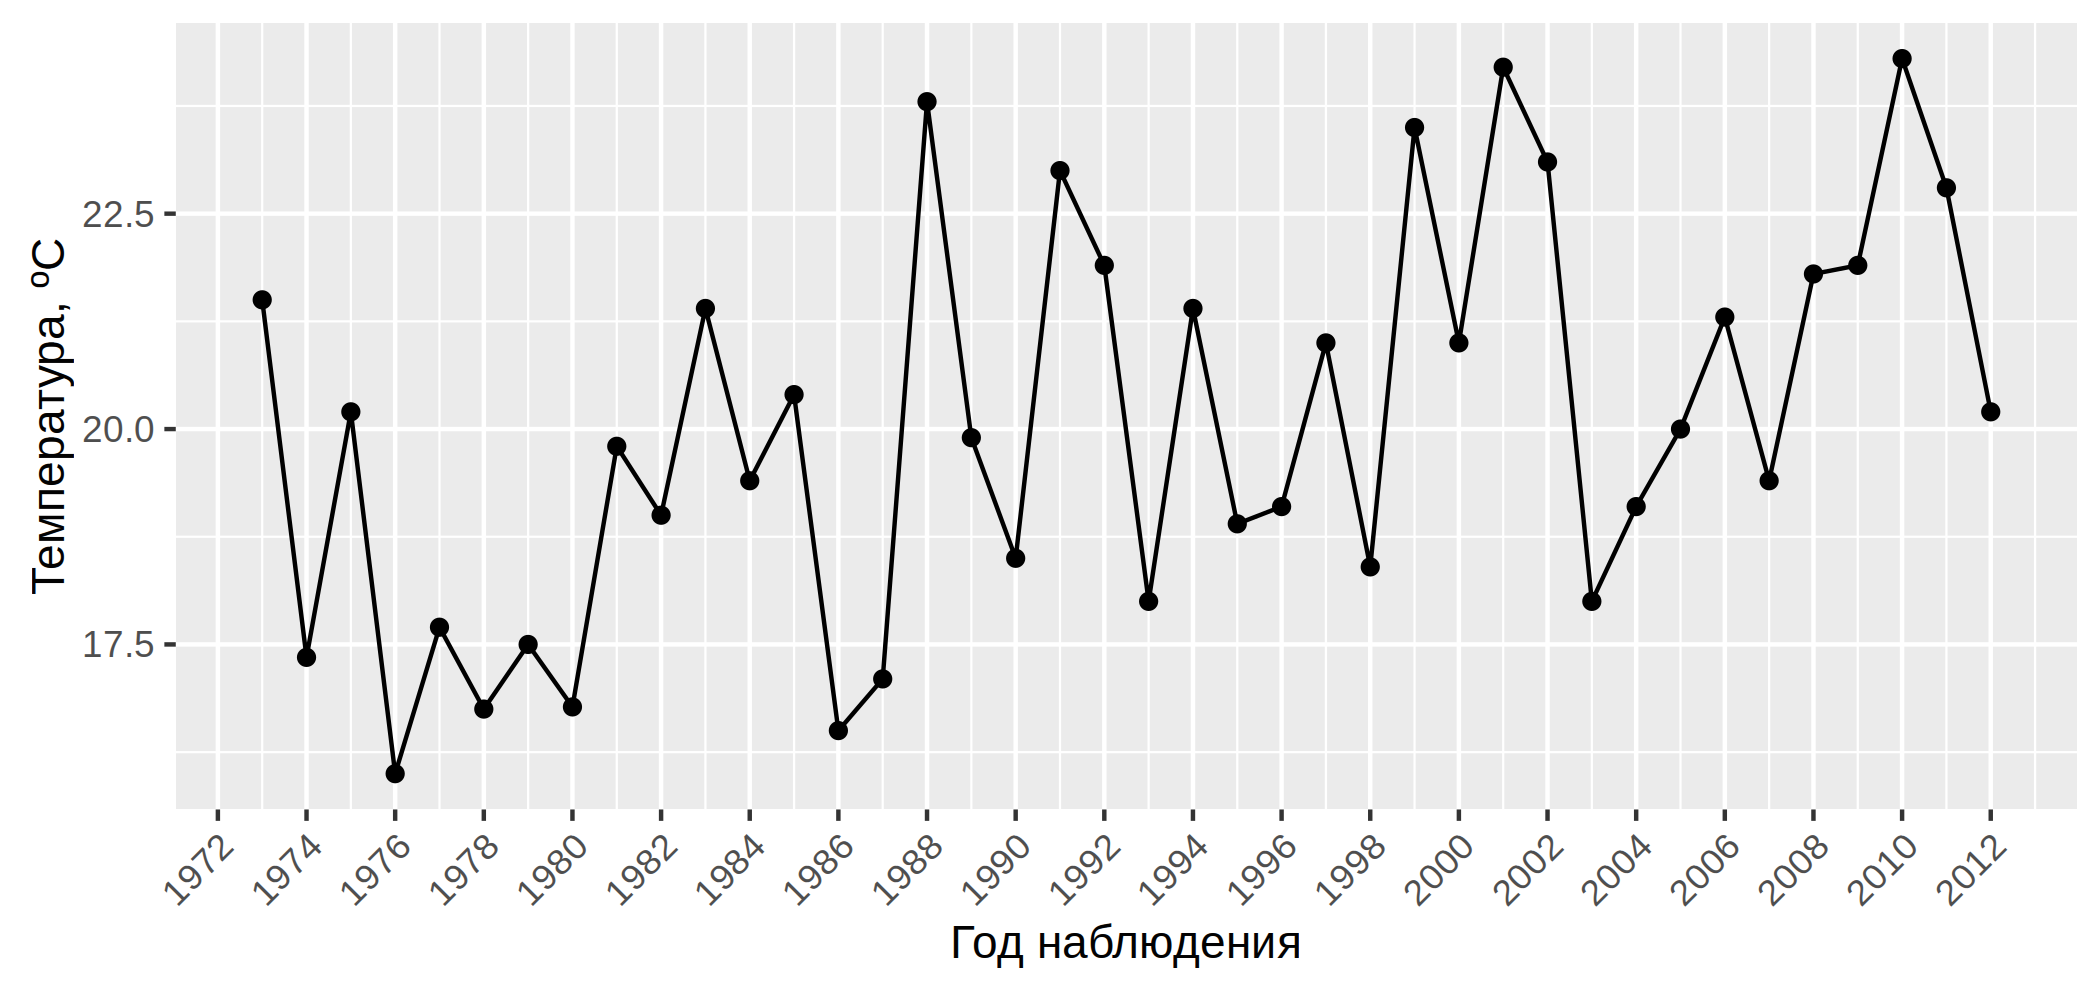
\includegraphics[width=1\linewidth]{../figures/source.png}}
\caption{График исходных данных}
\label{img:input}
\end{figure}

Следует отметить, что для непосредственного исследования в данном разделе были использованы наблюдения с 1975 по 2006 год. Наблюдения за 2007-2012 годы были намеренно исключены из исследования в целях дальнейшего оценивания результатов анализа и прогнозирования. Заметим, что работа, представленная в параграфах \ref{sec:basis}--\ref{sec:regr_analysis}, была также проделана и для всей выборки. Так как поведение целой выборки сохранилось в уменьшенной, то, без потери общности, будем считать её исходной. Обозначим её $ x(t), t = \overline{1, n} $, где $ n $ --- объём выборки, в данном случае равный $ \characteristic{original}{n} $.

Начнём исследование временного ряда с вычисления описательных статистик. \textbf{R} предоставляет в пакете \textit{base} различные функции для расчетов базовых статистик. Также, в различных пакетах можно найти другие интересующие функции, как статистические, так и математические. Но в целях удобства, компактности и контроля за функциональностью на основе \cite{Eliseeva1995, Cramer1997} мной был написан модуль \textit{dstats}, представленный в приложении \ref{c:listings} листинге \ref{lst:dstats}. Данный модуль позволяет вычислять все рассмотренные в данной работе описательные статистики. Полученные результаты для исходных данных отображены в таблице \ref{table:dstats}.

% latex table generated in R 3.1.2 by xtable 1.7-4 package
% Fri May 15 14:18:49 2015
\begin{table}[ht]
\centering
\begin{tabular}{rr}
  \hline
 & Значение \\ 
  \hline
Среднее & 19.88 \\ 
  Медиана & 19.80 \\ 
  Нижний квартиль & 18.20 \\ 
  Верхний квартиль & 21.40 \\ 
  Минимум & 16.00 \\ 
  Максимум & 24.20 \\ 
  Размах & 8.20 \\ 
  Квартильный размах & 3.20 \\ 
  Дисперсия & 4.92 \\ 
  Стандартное отклонение & 2.22 \\ 
  Коэффициент вариации & 24.75 \\ 
  Стандартная ошибка & 0.37 \\ 
  Асимметрия & 0.18 \\ 
  Ошибка асимметрии & 0.40 \\ 
  Эксцесс & -0.79 \\ 
  Ошибка эксцесса & 0.78 \\ 
   \hline
\end{tabular}
\caption{Описательные статистики для наблюдаемых температур.} 
\label{table:dstats}
\end{table}


Рассмотрим подробнее некоторые полученные статистики.

Как видно из таблицы, \textit{средняя} температура в июле месяце за период с 1975 по 2006 составляет приблизительно 20ºС.

\textit{Коэффициент вариации} в нашем случае равен $ \descriptive{original}{coef-var} $. Из этого следует, что выборку можно считать однородной, так как полученное значение является меньшим 33\% \cite{Eliseeva1995}.

\textit{Коэффициент асимметрии} --- мера симметричности распределения. Полученное значение: $ \descriptive{original}{skew} $. Данное значение говорит о незначительной правосторонней асимметрии распределения. То есть о том, что выборочное распределение можно считать близким к нормальному \cite{Bulmer1979Principles}.

\textit{Коэффициент эксцесса} в рассматриваемом случае равен $ \descriptive{original}{kurtosis}$. Так как коэффициент эксцесса нормального распределения равен $ 0 $, то в данном случае можно говорить о пологости пика распределения выборки по отношению к нормальному распределению \cite{Bulmer1979Principles}.

С помощью тестовых статистик для коэффициента асимметрии и эксцесса \cite[с.85-89]{Cramer1997}, проверим значимость полученных значений для генеральной совокупности. Для этого в модуле \textit{dstats} мной реализованы функции \textit{dstats.test.skew} и \textit{dstats.test.kurtosis}:

Полученная тестовая статистика для коэффициента асимметрии:
\begin{equation*}
	Z_{A_S} = \frac{A_S}{SES} = \descriptive{original}{test-skew}.
\end{equation*}
Данное значение попадает под случай $\vert Z_{A_S} \vert \le 2$, а значит, выборочный коэффициент асимметрии не является значимым. Из чего, в свою очередь, следует, что по нему нельзя судить о коэффициенте асимметрии генеральной совокупности \cite[с.85]{Cramer1997}.

Полученная тестовая статистика для коэффициента эксцесса:
\begin{equation*}
	Z_K = \frac{K}{SEK} = \descriptive{original}{test-kurtosis}.
\end{equation*}
Данное значение попадает под случай $\vert Z_K \vert \le 2$, а значит, в данном случае выборочный коэффициент эксцесса не является значимым и нельзя ничего сказать о коэффициенте эксцесса генеральной совокупности \cite[с.89]{Cramer1997}.

% TODO: стоит переписать, т.к. эксцесс получился не очень и убрали параграф с отдельно ОС
Из полученных результатов следует отметить, что коэффициенты асимметрии и эксцесса, указывают на некоторое отклонение выборочного распределения от нормального закона. Но при этом, из-за недостаточного объёма выборки, по этим коэффициентам нельзя судить о соответствующих коэффициентах генеральной совокупности.

В \textbf{R} можно найти различные пакеты, позволяющие строить разнообразные гистограммы, диаграммы рассеяния, вероятностные графики, линейные графики, диаграммы диапазонов, размахов, круговые диаграммы, столбчатые диаграммы, последовательные графики и т.д., позволяющие увидеть специфику данных. В процессе работы в пакете \textbf{R} использовались источники \cite{Kabacoff2009R, Teetor2011RCook, Chang2012RGraph}.

С помощью функции пакета \textit{ggplot2} построим гистограмму для отображения вариационного ряда исходных данных \cite{Chang2012RGraph}. Гистограммы позволяют увидеть, как распределены значения переменных по интервалам группировки, то есть как часто переменные принимают значения из различных интервалов. А также, что бывает более важным, позволяет сделать предположение о разновидности распределения. Для вычисления интервалов разбиения воспользуемся \textit{формулой Стерджеса}. Из \cite{Sturges1926Choice} количество интервалов разбиения рассчитывается по формуле:
\begin{equation}
\label{eq:sturges}
	k = \lceil log_{2}n \rceil + 1 = \lceil log_{2} \characteristic{original}{n} \rceil + 1 = \characteristic{original}{sturges}.
\end{equation}

Так как по гистограмме можно визуально предположить близость выборочного распределения к нормальному распределению, нанесём на график кривую плотности нормального распределения (рисунок \ref{img:histogram_fitted}).
\begin{figure}[ht]
	\center{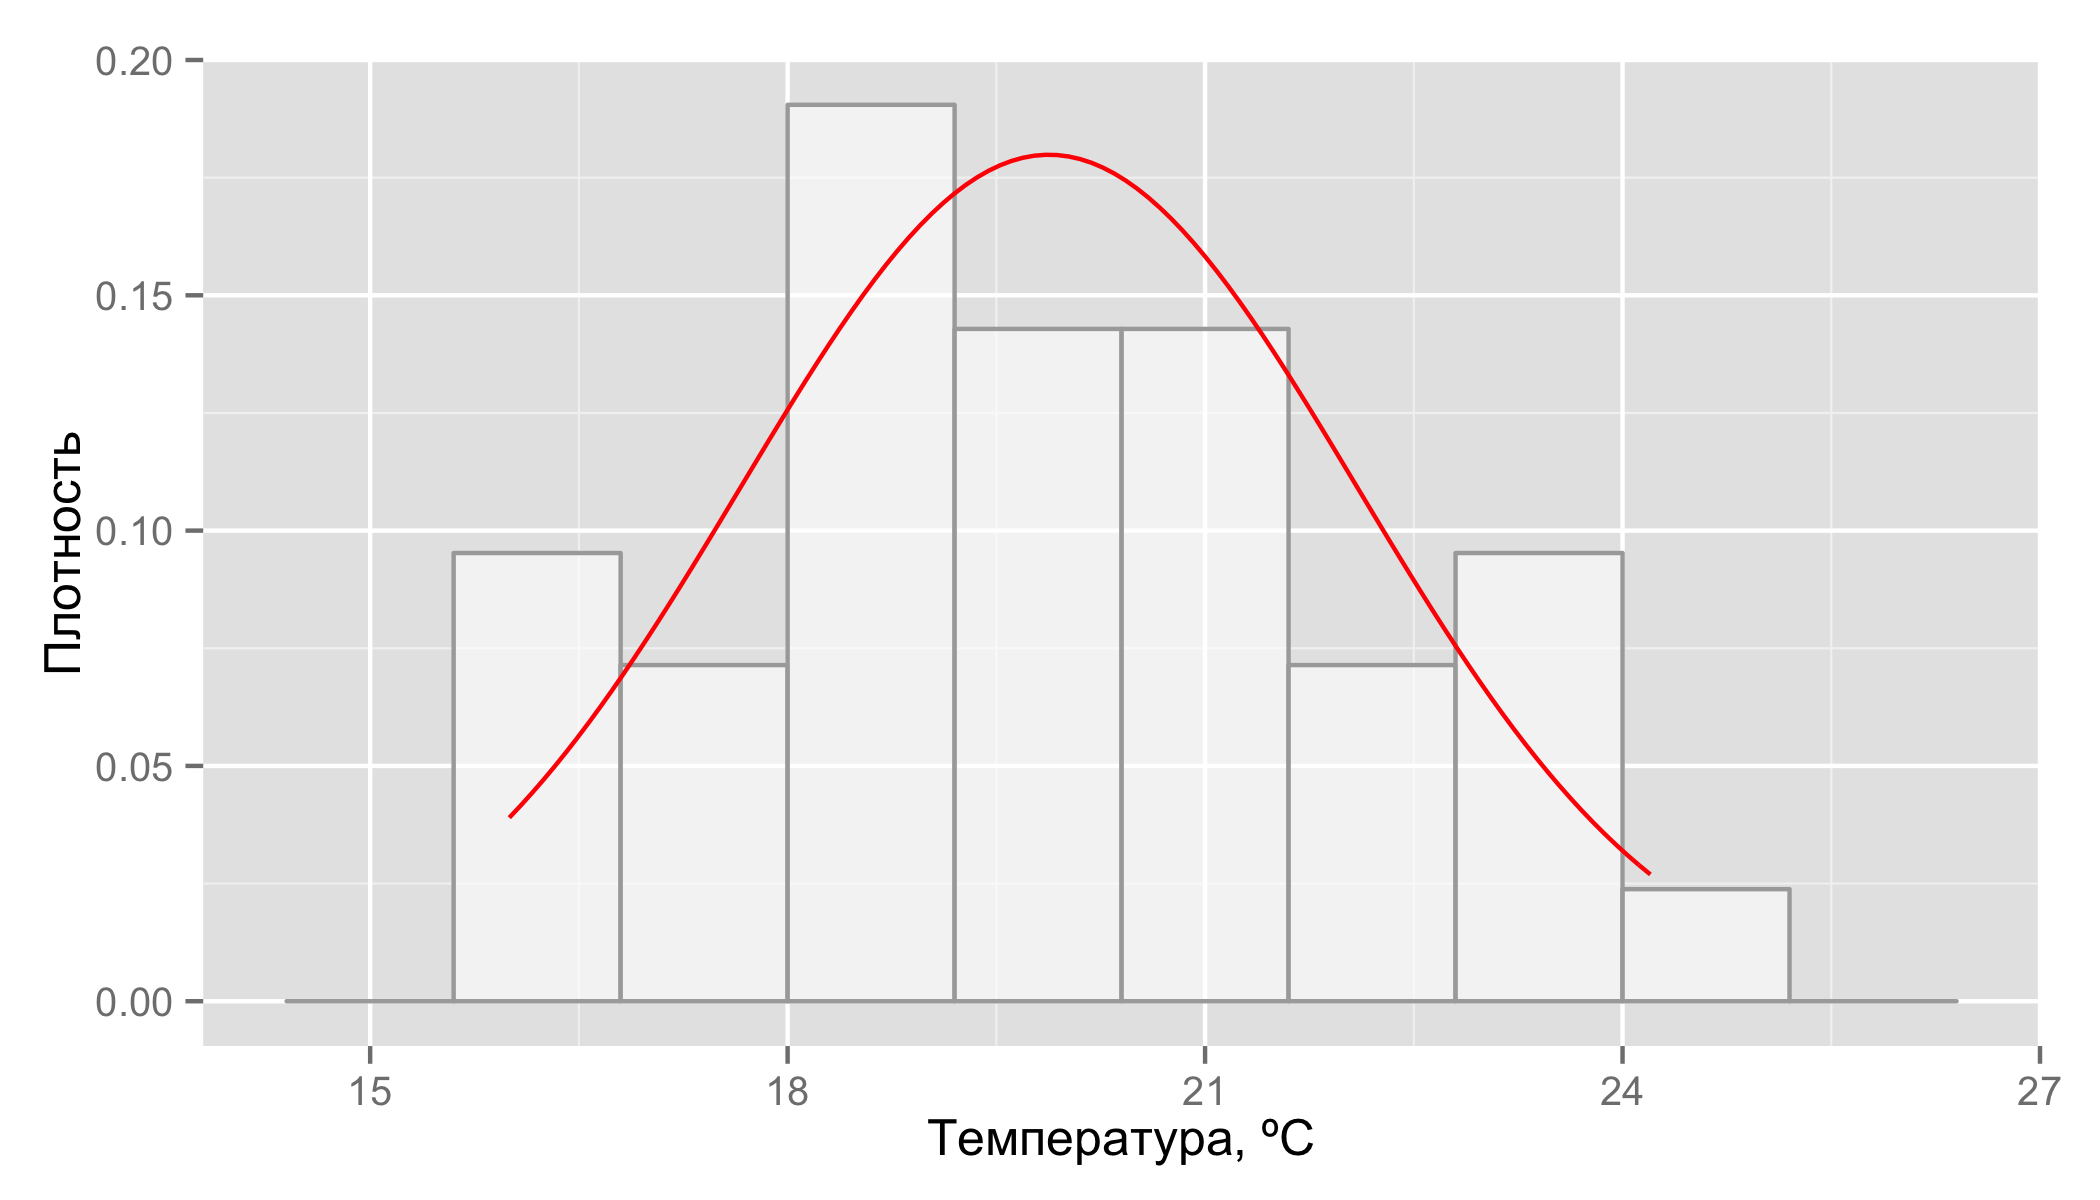
\includegraphics[width=1\linewidth]{../figures/original/histogram.png}}
\caption{Гистограмма наблюдаемых температур с кривой плотности нормального распределения $\mathcal{N}(19.77, 5.12)$}
\label{img:histogram_fitted}
\end{figure}
Проанализируем эту гистограмму. Во-первых, на ней наглядно представлены показатели асимметрии и эксцесса, полученные на этапе вычисления описательных статистик. Таким образом показывает отношение выборочного распределения к нормальному с параметрами \normaldistr.

Следует отметить согласованность полученных описательных статистик с полученной гистограммой. Во-первых, по коэффициенту асимметрии мы предположили о близости распределения к симметричному. Это подтверждается гистограммой: на ней можно заметить небольшую скошенность вправо, что также согласовывается со знаком коэффициента. Во-вторых, коэффициент эксцесса указывал на пологость пика распределения. Данное заключение подтверждается кривой плотности --- она имеет чуть более растянутую колоколообразную форму.

Другим часто используемым графическим способом проверки характера распределения данных является построение т.н. \textit{графиков квантилей} (\textit{Q-Q plots}, \textit{Quantile-Quantile plots}). На таких графиках изображаются квантили двух распределений --- эмпирического (т.е. построенного по анализируемым данным) и теоретически ожидаемого нормального распределения. При нормальном распределении проверяемой переменной точки на графике квантилей должны выстраиваться в прямую линию, исходящую под улом 45 градусов из левого нижнего угла графика. Графики квантилей особенно полезны при работе с небольшими по размеру совокупностями, для которых невозможно построить гистограммы, принимающие какую-либо выраженную форму.

В ходе данной работы была написана функция \textit{ggqqp}, с помощью которой построен график \ref{img:qqnorm}.
\begin{figure}[ht]
	\center{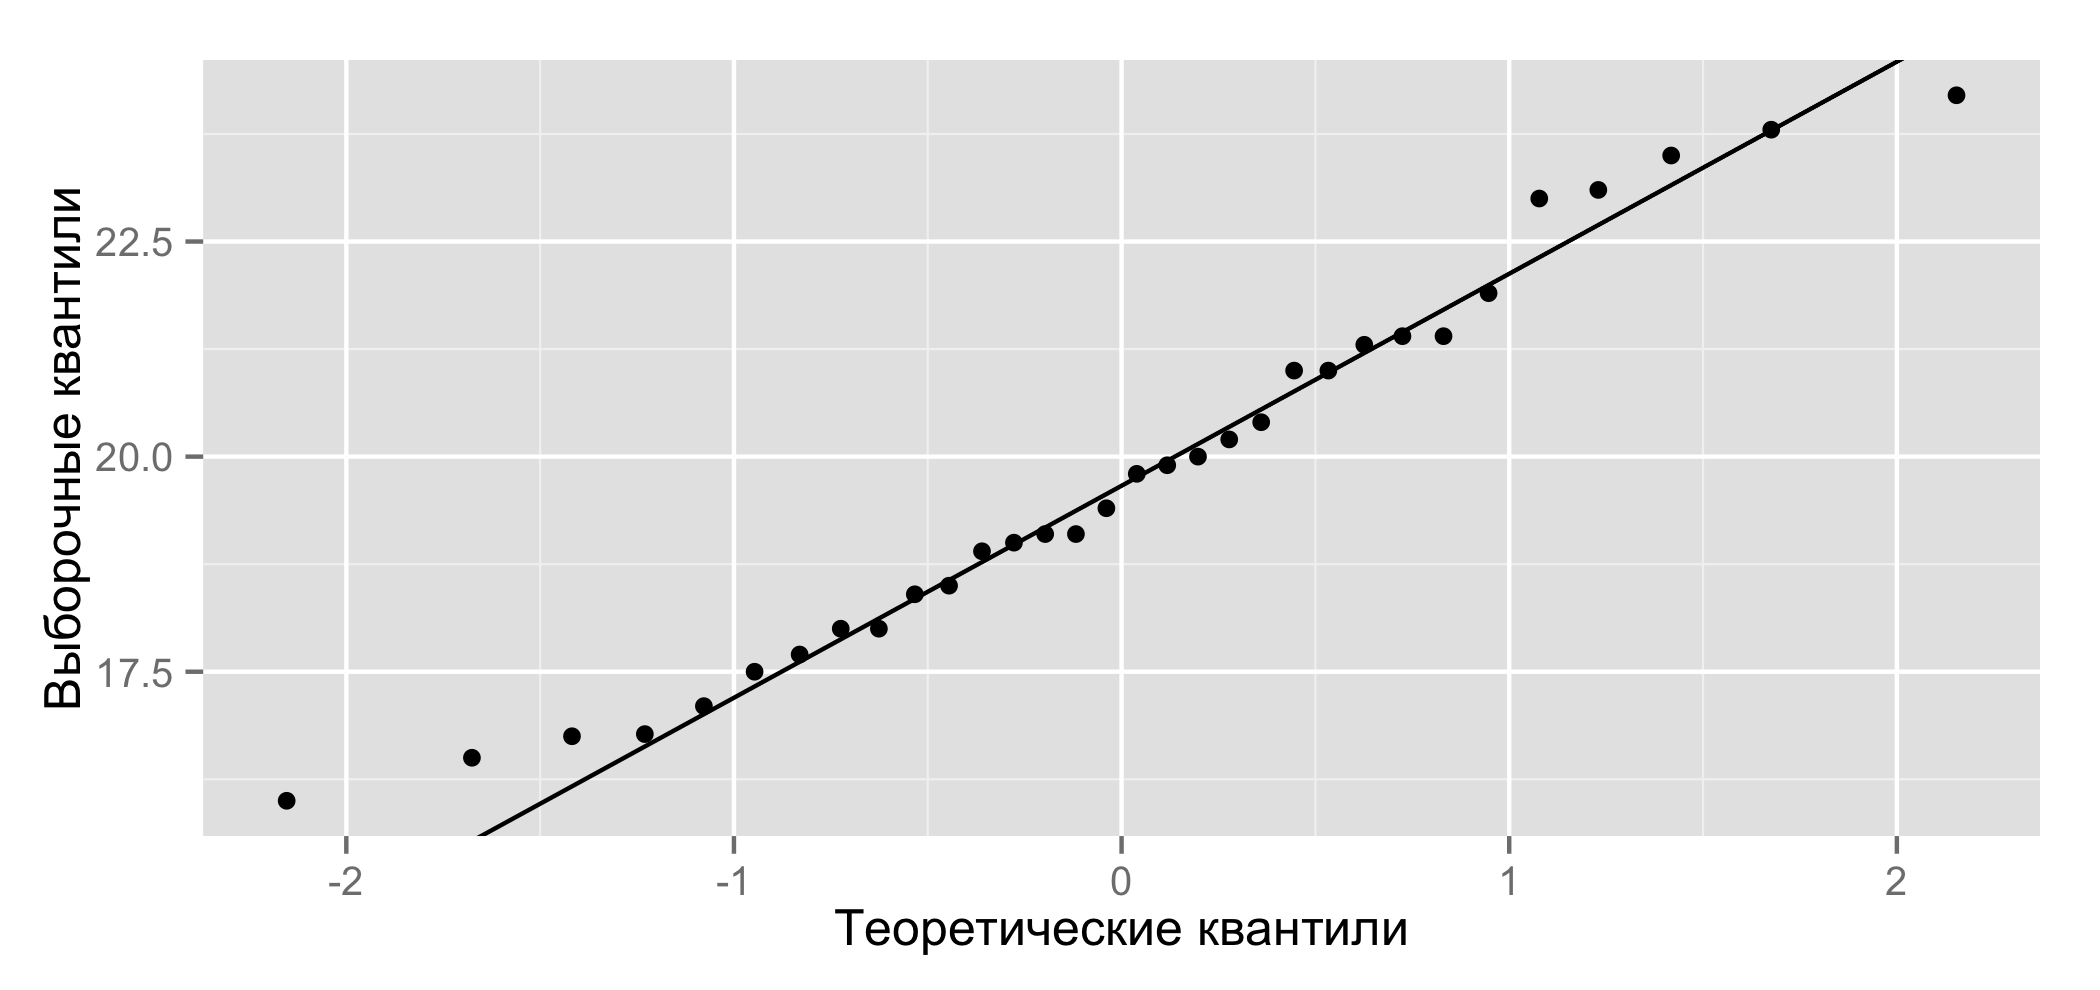
\includegraphics[width=1\linewidth]{../figures/original/quantile.png}}
\caption{График квантилей для наблюдаемых температур}
\label{img:qqnorm}
\end{figure}
На этом графике можно визуально обнаружить аномальное положение наблюдаемых значений по отношению к нормальному распределению. В данном случае отклонения можно наблюдать на концах рассматриваемого промежутка. Остальные значения образуют отчетливую прямую. Это следует интерпретировать как близость выборочного распределения к нормальному с параметрами \normaldistr.

Далее следует проверить полученные результаты и предположения с помощью некоторых формальных тестов. Существует целый ряд статистических тестов, специально разработанных для проверки нормальности выборочного распределения. В общем виде проверяемую при помощи этих тестов нулевую гипотезу можно сформулировать следующим образом: ``Анализируемая выборка происходит из генеральной совокупности, имеющей нормальное распределение''. Если получаемая при помощи того или иного теста вероятность ошибки $P$ оказывается меньше некоторого заранее принятого уровня значимости (например, $0.05$), нулевая гипотеза отклоняется.

В \textbf{R} реализованы практически все имеющиеся тесты на нормальность --- либо в виде стандарных функций, либо в виде функций, входящих в состав отдельных пакетов. Примером базовой функции является \textit{shapiro.test()}, при помощи которой можно выполнить широко используемый \textit{тест Шапиро-Уилка} \cite{Shapiro1972}. Из полученных в \textbf{R} результатов, статистика Шапиро-Уилка $ W = \test{original}{shapiro}{statistic} $. Вероятность ошибки $ p = \test{original}{shapiro}{p-value} > 0.05 $, а значит нулевая гипотеза не отвергается \cite{Kobzar2006}. Следовательно опровергнуть предположение на основе данного теста нельзя.

Попробуем опровергнуть наше предположение на основе проверки критерия $ \chi^2 $ Пирсона \cite{Gmurman2003}. Для этого воспользуемся пакетом \textit{nortest} и функцией \textit{pearson.test}. Из полученных в \textbf{R} результатов, статистика $\chi^2$ Пирсона $ P = \test{original}{pearson}{statistic}$. Вероятность ошибки $ p = \test{original}{pearson}{p-value} > 0.05 $, а значит нулевая гипотеза не отвергается. Следовательно опровергнуть предположение о нормальности на основе данного теста также нельзя. Проверим критерий: примем уровень значимости $\alpha = 0.05$, тогда из таблицы распределения $\chi^2$ найдём критическое значение критерия $P_{\textrm{кр}}(\alpha, k) = 43.8$. Отсюда следует, что

\begin{equation*}
	P < P_{\textrm{кр}}.
\end{equation*}

А значит, нулевую гипотезу при уровне значимости $\alpha = 0.05$ не отвергаем и подтверждаем сделанный вывод на основании вычисленной вероятности ошибки.

Воспользуемся для тех же целей критерием Колмогорова--Смирнова \cite{Mikulik2002}. Как в предыдущем случае воспользуемся представленной в пакете \textit{nortest} функцией \textit{ks.test}. Из полученных в \textbf{R} результатов, статистика Колмогорова-Смирнова $ D = \test{original}{ks}{statistic}$. Вероятность ошибки $ p = \test{original}{ks}{p-value} > 0.05 $, а значит нулевую гипотезу отвергнуть нельзя. Следовательно опровергнуть предположение о нормальности, как и в предыдущих случаях, также нельзя. Проверим критерий: примем так же уровень значимости $\alpha = 0.05$, тогда критическое значение $D_{\textrm{кр}}(\alpha) = 1.358$. Следовательно,
\begin{equation*}
	D < D_{\textrm{кр}}(\alpha),
\end{equation*}
и подтверждаем сделанные ранее заключения: нельзя отвергнуть нулевую гипотезу о нормальности выборочного распределения.

На данном этапе по полученным ранее результатам возникли подозрения о выбросах в исходной выборке. Выявление таких аномальных значений важно, так как их наличие, как правило, сильно влияет на всю выборку, в частности, на коэффициент корреляции. Проверим наличие выбросов с помощью статистических критериев. Для этих целей воспользуемся критерием Граббса \cite{Grubbs1950Sample}. Данный основан на предположении о нормальности исходных данных. То есть, перед применением данного критерия необходимо убедиться, что данные могут быть в разумных пределах аппроксимированы нормальным распределением \cite{grubbs}. Поскольку ранее высказано предположение о нормальности, воспользуемся им для определения наличия выбросов.

Полученные результаты проверки критерия Граббса: статистика $ G = \test{original}{grubbs}{statistic} $, вероятность ошибки $ p\textrm{-value} = \test{original}{grubbs}{p-value} $ --- что однозначно говорит нам о том, что следует отклонить альтернативную гипотезу $H_{1}$ и принять гипотезу $H_{0}$. Другими словами, это говорит о том, что в исходной выборке нету выбросов. А значит выборка однородна. Таким образом, подозрения о выбросах не подтвердились проверкой критерия.

В соответствии с результатами проверки критериев и на основе построенных гистограммы и графика квантилей, можно сделать заключение о том, что распределение температуры воды озера Баторино в июле 1975--2009 годов является близким к нормальному закону распределения с параметрами \normaldistr. При этом, обнаружены отклонения от нормальности, описываемые коэффициентами асимметрии и эксцесса. Следует также отметить, что эквивалентные результаты были получены и для всей выборки, до исключения последних наблюдений. При этом, отклонение от нормальности было менее выраженным. Таким образом, отклонение от нормальности можно считать следствием потери информации при исключении наблюдений из исходной выборки.

% subsection basis (end)

\subsection{Корреляционный анализ} % (fold)
\label{sec:corr_analysis}

Исследуем теперь зависимость температуры воды от времени, построив диаграмму рассеяния и вычислив коэффициент корреляции соответствующих переменных.

Диаграммы рассеяния используются для визуального исследования зависимости между двумя переменными. Если переменные сильно связаны, то множество точек данных принимает определённую форму. С помощью таких диаграмм можно наглядно изучить знак коэффициента корреляции. Если точки на диаграмме расположены хаотически, то это говорит о независимости рассматриваемых переменных. Если с ростом переменной $t$ возрастает переменная $x$ то имеет место положительная корреляция. Если же с ростом переменной $ t $ переменная $ x $ убывает, то это указывает на отрицательную корреляцию.
\begin{figure}[ht]
	\center{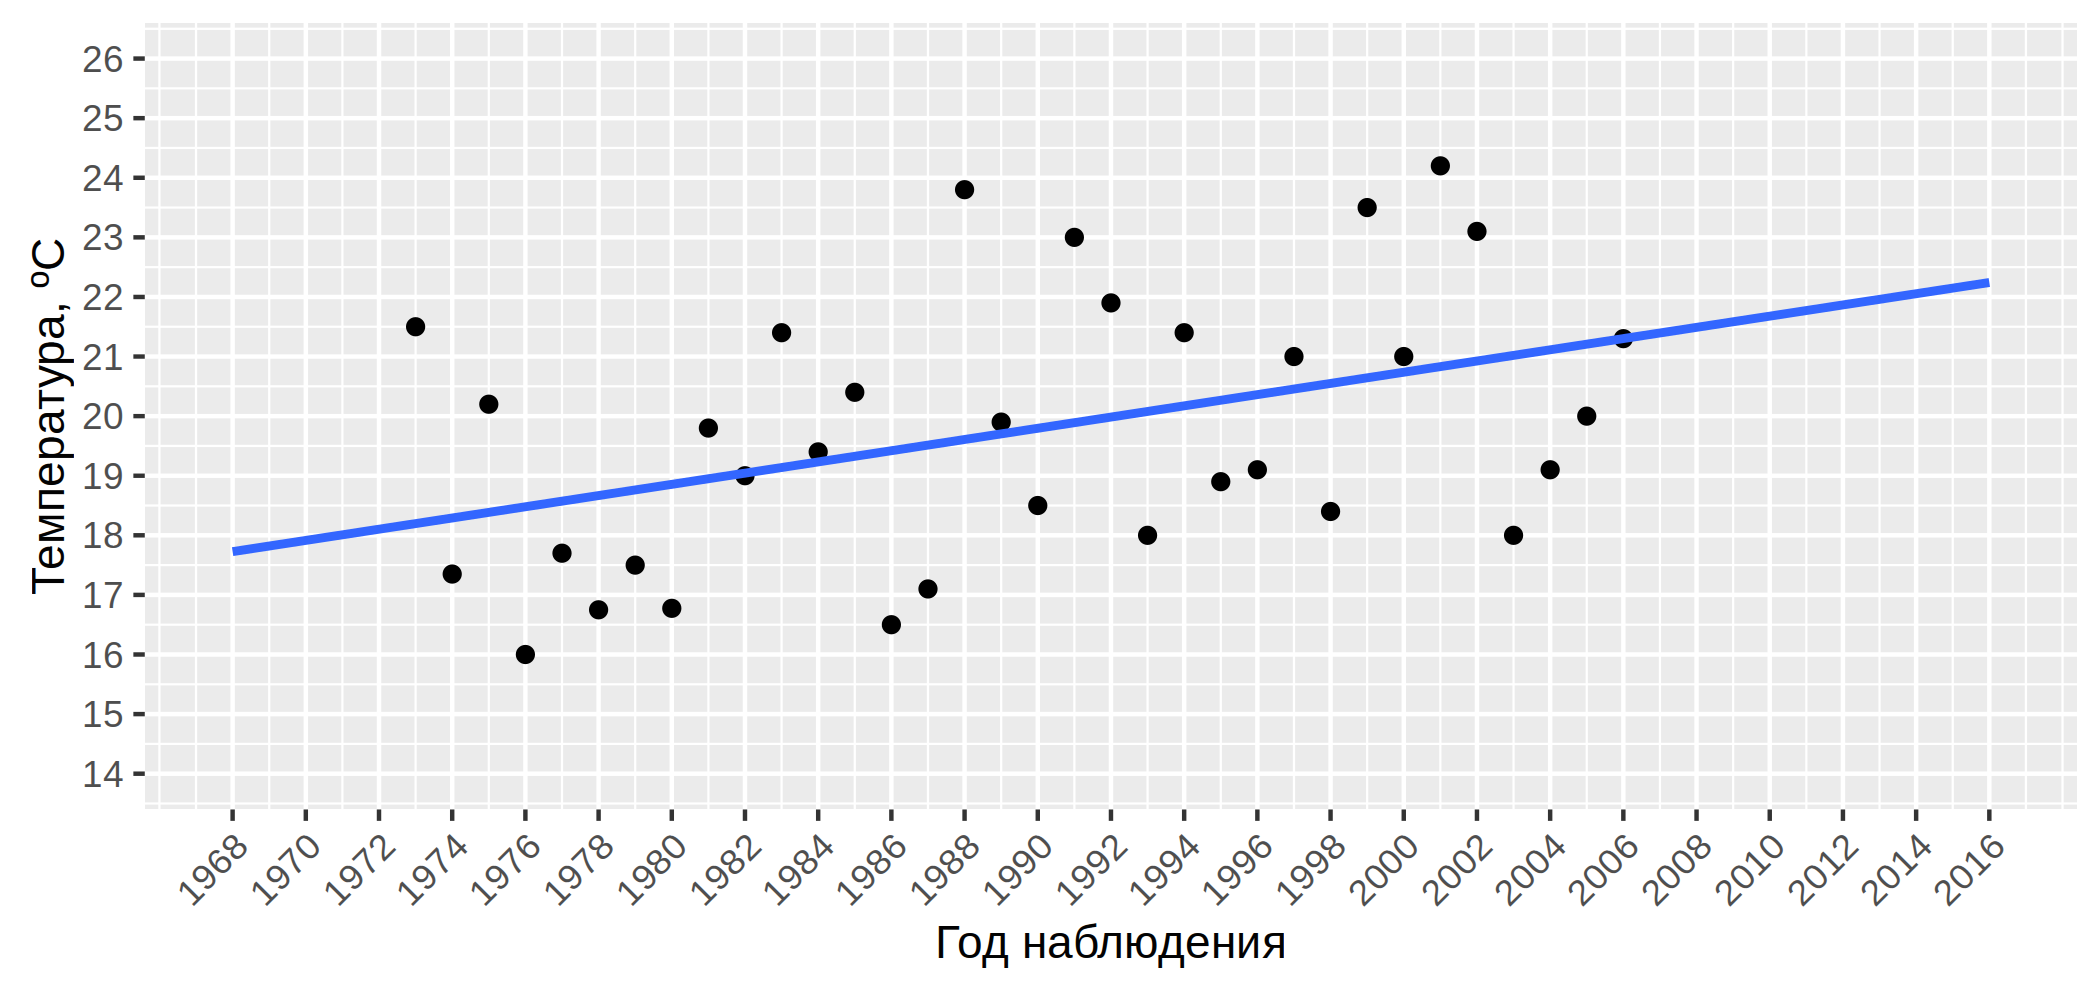
\includegraphics[width=1\linewidth]{../figures/original/scatterplot.png}}
\caption{Диаграмма рассеяния}
\label{img:scatterplot}
\end{figure}

Из рисунка \ref{img:scatterplot} видно, что точки образуют своеобразное <<облако>>, ориентированное по вверх, то есть присутствует некая зависимость между рассматриваемыми переменными. Также, данная диаграмма наглядно показывает силу этой зависимости: так как точки не образуют чёткой формы, а разбросаны относительно линии, то можно говорить о наличии умеренной корреляции.

Проверим полученные результаты подробнее. Из расчётов в \textbf{R}, коэффициент корреляции $ r_{xt} = \characteristic{original}{correlation} $. Этим подтверждаются наши выводы из диаграммы рассеяния о положительной корреляции, поскольку полученный коэффициент корреляции является положительным и присутствует умеренная зависимость: $r_{xt} \approx 0.5$.

Проверим значимость полученного выборочного коэффициента корреляции с помощью критерия Стьюдента:
\begin{equation*}
	T_{\textrm{набл}} = \frac{r_{xt} \sqrt{n - 2}}{\sqrt{1 - r_{xt}^2}} \approx \test{original}{student}{statistic}.
\end{equation*}
Рассмотрим уровень значимости $\alpha = 0.05$. Число степеней свободы $k = n - 2 = \test{original}{correlation}{df}$. Тогда из таблицы критических точек распределения Стьюдента $t_\textrm{кр}(\alpha, k) \approx \test{original}{student}{df}$. Следовательно,
\begin{equation*}
	T_{\textrm{набл}} > t_\textrm{кр}(\alpha, k).
\end{equation*}
Значит нулевую гипотезу о равенстве нулю коэффициента корреляции генеральной совокупности следует отклонить \cite{Eliseeva1995}.

Также оценим значимость с помощью возможностей пакета \textbf{R} и функции \textit{cor.test}. Представленная функция позволяет с помощью различных методов выполнять проверки значимости выборочного коэффициента корреляции. Воспользуемся проверкой теста методом Пирсона. Из результатов её выполнения статистика $ t = \test{original}{correlation}{statistic} $, количество степеней свободы $ df = \test{original}{correlation}{df} $ и вероятность ошибки $p = \test{original}{correlation}{p-value} < 0.05$, следовательно это говорит о том, что необходимо отвергнуть гипотезу $H_0: r = 0$.

Результаты обоих подходов в проверке значимости совпали. Другими словами, выборочный коэффициент значимо отличается от нуля, т.е. температура воды и время при уровне значимости $\alpha = 0.05$ имеют зависимость.

Следовательно, в рассматриваемом случае можно говорить о присутствии значимой корреляции между температурой воды в озере Баторино и временем. Что говорит росте температуры окружающей среды с момента начала наблюдений.

% subsection corr_analysis (end)

\subsection{Регрессионный анализ} % (fold)
\label{sec:regr_analysis}

Для введения последующих понятий анализа временных рядов воспользуемся \cite{Eddows1997}.

В отличие от анализа случайных выборок, анализ временных рядов основывается на предположении, что последовательные значения в исходных данных наблюдаются через равные промежутки времени. Во временных рядах выделяют три составляющие:
\begin{enumerate}
	\item \textit{Тренд (тенденция развития)} --- эволюционная составляющая, которая характеризует общее направление развития изучаемого явления и связанна с действием долговременных факторов развития.
	\item \textit{Циклические, сезонные колебания} --- это составляющие, которые проявляются как отклонения от основной тенденции развития изучаемого явления, и связанны с действие краткосрочных, систематических факторов развития.
	\item \textit{Нерегулярная случайная составляющая (ошибка)}, являющаяся результатом действия второстепенных факторов развития.
\end{enumerate}
Первые два типа компонент представляют собой детерминированные составляющие. Случайная составляющая образована в результате суперпозиции некоторого числа внешних факторов.

По типу взаимосвязи вышеперечисленных составляющих ряда динамики можно построить следующие модели временных рядов:
\begin{itemize}
	\item Аддитивная модель: $ x = y + k + s + \varepsilon $;
	\item Мультипликативная модель: $x = y \times k \times s \times \varepsilon$,
\end{itemize}
где $y, k, s, \varepsilon$ --- тренд, циклическая, сезонная и нерегулярная составляющие соответственно.

Аддитивной модели свойственно то, что характер циклических и сезонных колебаний остаётся постоянным. В мультипликативной модели характер циклических и сезонных колебаний остаётся постоянным только по отношению к тренду (т.е. значения этих составляющих увеличиваются с возрастанием значений тренда).

По причине того, что в данном случае мы рассматриваем один месяц в году на протяжении длительного периода, будем считать, что в рассматриваемом временном ряде циклическая и сезонная составляющие отсутствуют.

При проведении корреляционного анализа, на графике \ref{img:scatterplot} был замечен явно выраженный линейный рост значений со временем. Что впоследствии было подтверждено критериями. Из этого следует, что уравнение тренда имеет вид:
\begin{equation*}
	y(t) = at + b,
\end{equation*}
где $ a, b \in \mathbb{R}, t = \overline{0, n - 1} $ -- некоторые коэффициенты, $ n $ --- объем выборки.

Продолжая рассуждение, как наблюдение из графика, можно отметить, что не происходит увеличения амплитуды колебаний с течением времени. А значит, искомая модель является аддитивной. Из всего вышесказанного можно заключить, что модель исходного временного ряда имеет вид:
\begin{equation*}
	x = y + \varepsilon,
\end{equation*}
где $ y $ -- тренд, $ \varepsilon $ - нерегулярная составляющая.

В \textbf{R} реализованы функции, позволяющие подгонять линейные модели к исследуемым данным \cite{Shumway2006Time}. Одной из таких функций является \textit{lm(Fitting Linear Model)} \cite[c.178]{Kabacoff2009R}. Она позволяет получить коэффициенты линии регрессии. Таким образом, можно вычислить одну из искомых компонент -- тренд. И как следствие, после его удаления из исходных данных, получим нерегулярную составляющую $ \varepsilon(t) $. Коэффициенты, полученные с помощью данной функции представлены в \eqref{eq:regr_coeff}.
\begin{equation}
\label{eq:regr_coeff}
	a = \characteristic{original}{sign-a}, \quad b = \characteristic{original}{sign-b}.
\end{equation}
Следует отметить, что в пакете \textbf{STATISTICA} похожая процедура была проведена для всей выборки с помощью инструмента \textit{Trend Subtract}, результаты которой согласуются с полученными в \textbf{R} коэффициентами.

Таким образом получена линейная модель, описывающая тенденцию развития:
\begin{equation}
\label{eq:regr}
	y(t) = at + b = \characteristic{original}{sign-a}t + \characteristic{original}{sign-b}
\end{equation}

На основе полученной линейной модели \eqref{eq:regr}, построим ряд остатков, удалив тренд из исходного ряда. Полученный ряд представлен в приложении \ref{c:app_results} в таблице \ref{table:residuals} и графически на рисунке \ref{img:ts_detrended}.
\begin{figure}[ht]
	\center{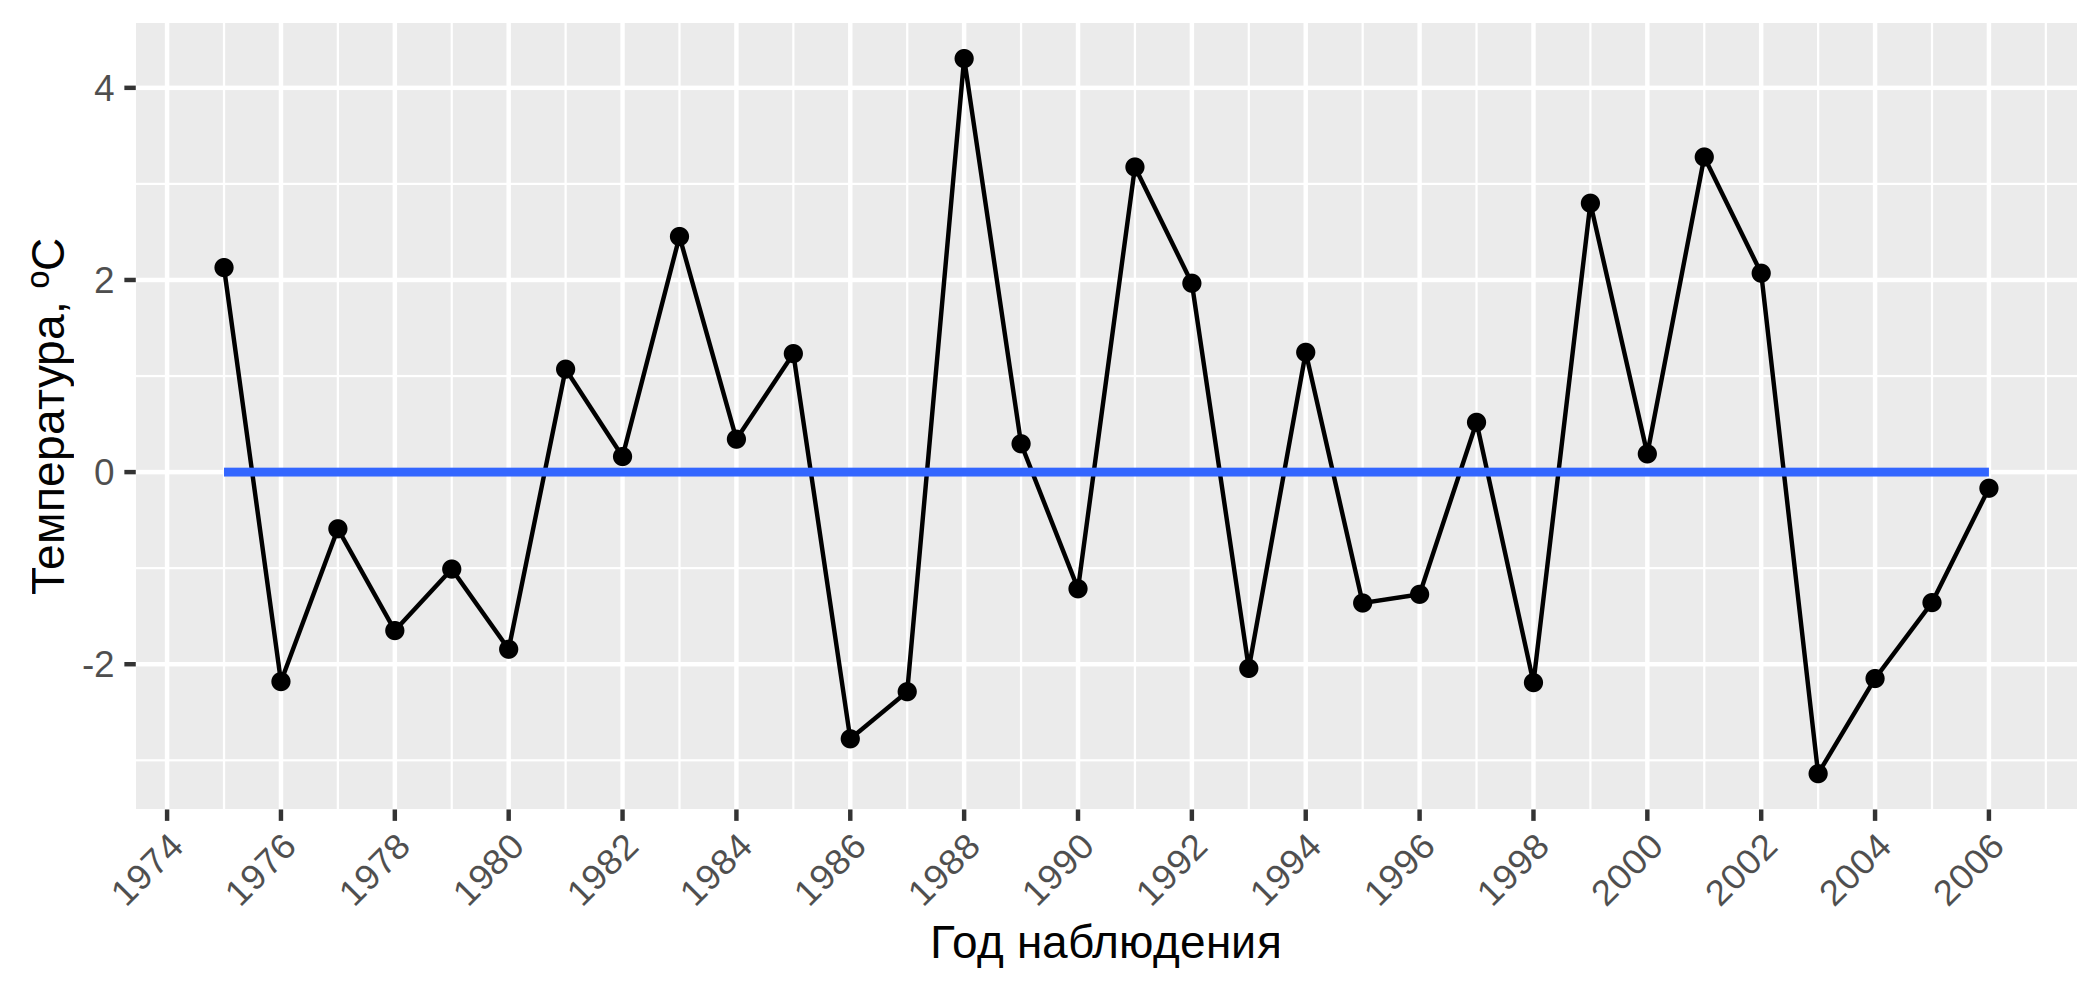
\includegraphics[width=1\linewidth]{../figures/residual/time-series.png}}
\caption{Нерегулярная составляющая $ \varepsilon(t) $}
\label{img:ts_detrended}
\end{figure}

Проведём анализ полученной регрессионной модели. Для этого проверим значимость полученных коэффициентов регрессии и оценим адекватность вычисленной регрессионной модели.

Рассчитаем вспомогательные величины, воспользовавшись \cite{Eddows1997}. Дисперсия отклонения
\begin{equation*}
	\sigma_{\varepsilon}^2 \approx \characteristic{original}{sign-vardev},
\end{equation*}
стандартные случайные погрешности параметров $a, b$:
\begin{equation*}
	\sigma_{a} \approx \characteristic{original}{sign-errorA}, \quad \sigma_{b} \approx \characteristic{original}{sign-errorB}.
\end{equation*}

Воспользуемся критерием значимости коэффициентов линейной регрессии \cite{Eliseeva1995}. Примем уровень значимости $\alpha = 0.05$, тогда
\begin{equation*}
	T_{a} = \characteristic{original}{sign-studentA}, \quad T_{b} = \characteristic{original}{sign-studentB}.
\end{equation*}

Число степеней свободы $k = \characteristic{original}{sign-df}$, $t_{\textrm{кр}}(k, \alpha) = \characteristic{original}{sign-critical}$.

\begin{itemize}
	\item $\vert T_{a} \vert > t_{\textrm{кр}}$ $\Rightarrow$ коэффициент $a$ значим.
	\item $\vert T_{b} \vert > t_{\textrm{кр}}$ $\Rightarrow$ коэффициент $b$ значим.
\end{itemize}
Следовательно, при уровне значимости $\alpha = 0.05$, коэффициенты линейной регрессии являются значимыми.

Оценим адекватность полученной регрессионной модели. Дисперсия модели:
\begin{equation*}
	\overline{\sigma^2} \approx \characteristic{original}{adeq-var_}.
\end{equation*}

Остаточная дисперсия:
\begin{equation*}
	\overline{D} \approx \characteristic{original}{adeq-resvar}.
\end{equation*}

Воспользуемся F-критерием Фишера. Пусть уровень значимости $\alpha = 0.05$,
\begin{equation*}
	F_{\textrm{крит}} \approx \characteristic{original}{adeq-statistic},
\end{equation*}
при степенях свободы $v_1 = 1, v_2 = \characteristic{original}{sign-df}, F_{\textrm{табл}}(v_1, v_2, \alpha) = \characteristic{original}{adeq-critical}$.

\begin{equation*}
	F_{\textrm{крит}} > F_{\textrm{табл}}.
\end{equation*}
Следовательно, при уровне значимости $\alpha = 0.05$, регрессионная модель является адекватной.

Рассчитаем коэффициент детерминации:
\begin{equation*}
	\eta_{x(t)}^2 \approx \characteristic{original}{adeq-determination}.
\end{equation*}

Проверим отклонение от линейности: $\eta_{x(t)}^2 - r_{xt}^{2} \approx \characteristic{original}{adeq-linearity} \le 0.1$. Следовательно отклонение от линейности незначительно. Но при этом коэффициент детерминации оказался не высоким($<0.7$), это говорит о том, что построенная регрессионная модель не описывает в достаточной мере поведение временного ряда. Это, в свою очередь, может значить, что изменение температуры зависит не только от времени, но ещё и от каких-то других, неучтённых, факторов.

Тем не менее, попробуем построить прогноз по полученной модели. Вычисленные прогнозные значения на 2007-2012 годы для сравнения отображены в таблице \ref{table:prediction_trend}:
% latex table generated in R 3.1.3 by xtable 1.7-4 package
% Thu May 21 14:09:02 2015
\begin{table}[ht]
\centering
\begin{tabular}{rrrr}
  \hline
 & Год & Актуальное & Прогнозное \\ 
  \hline
1 & 2007 & 19.40 & 18.07 \\ 
  2 & 2008 & 21.80 & 18.18 \\ 
  3 & 2009 & 21.90 & 18.29 \\ 
  4 & 2010 & 24.30 & 18.40 \\ 
  5 & 2011 & 22.80 & 18.51 \\ 
  6 & 2012 & 20.20 & 18.62 \\ 
   \hline
\end{tabular}
\caption{Сравнение прогнозных значений (тренда)} 
\label{table:prediction_trend}
\end{table}


Имеющееся отклонение прогнозов от реальных данных ещё раз подтверждает, что построенная модель временного ряда обладает невысокой точностью. И поэтому необходимо её улучшать другими методами.

% TODO Окончательно сказать, что тут использовалась СТАСТИСТИКА или где-нибудь в заключении

% subsection regr_analysis (end)

\subsection{Анализ остатков} % (fold)
\label{sub:analysis_residuals}

Проанализируем полученную на этапе регрессионного анализа нерегулярную составляющая $\varepsilon$. Для этого проверим свойства, которым она должна удовлетворять:
\begin{enumerate}
	\item Математическое ожидание $\varepsilon$ равно $ 0 $;
	\item Дисперсия $\varepsilon$ постоянна для всех значений;
	\item Остатки независимы и нормально распределены.
\end{enumerate}
Вычислим описательные статистики для остатков. Полученные результаты проследим по таблице \ref{table:residuals_dstats}.
% latex table generated in R 3.1.2 by xtable 1.7-4 package
% Mon Mar  2 02:32:46 2015
\begin{table}[ht]
\centering
\begin{tabular}{rr}
  \hline
 & Значение \\ 
  \hline
Среднее & -0.00 \\ 
  Медиана & 0.14 \\ 
  Нижний квартиль & -1.80 \\ 
  Верхний квартиль & 1.28 \\ 
  Минимум & -2.99 \\ 
  Максимум & 4.33 \\ 
  Размах & 7.32 \\ 
  Квартильный размах & 3.07 \\ 
  Дисперсия & 3.84 \\ 
  Стандартное отклонение & 1.96 \\ 
  Коэффициент вариации & 0.00 \\ 
  Стандартная ошибка & 0.33 \\ 
  Асимметрия & 0.42 \\ 
  Ошибка асимметрии & 0.40 \\ 
  Эксцесс & -0.77 \\ 
  Ошибка эксцесса & 0.78 \\ 
   \hline
\end{tabular}
\caption{Описательные статистики остатков} 
\label{table:residuals_dstats}
\end{table}


Как видно из таблицы \ref{table:residuals_dstats}, среднее значение равно нулю. При этом коэффициенты асимметрии($ A_S = \descriptive{residual}{skew} $) и эксцесса($ K = \descriptive{residual}{kurtosis} $) указывают на большее отклонение распределения остатков от нормального закона.

Построим гистограмму и график квантилей для проверки последних заключений. Построенная гистограмма (приложение \ref{c:graphs}, рисунок \ref{img:resid_hist}) наглядно демонстрирует полученные в таблице \ref{table:residuals_dstats} коэффициенты асимметрии и эксцесса.

Как и в случае исходных данных график квантилей позволяет наглядно оценить близость к нормальному распределению.
\begin{figure}[ht]
	\center{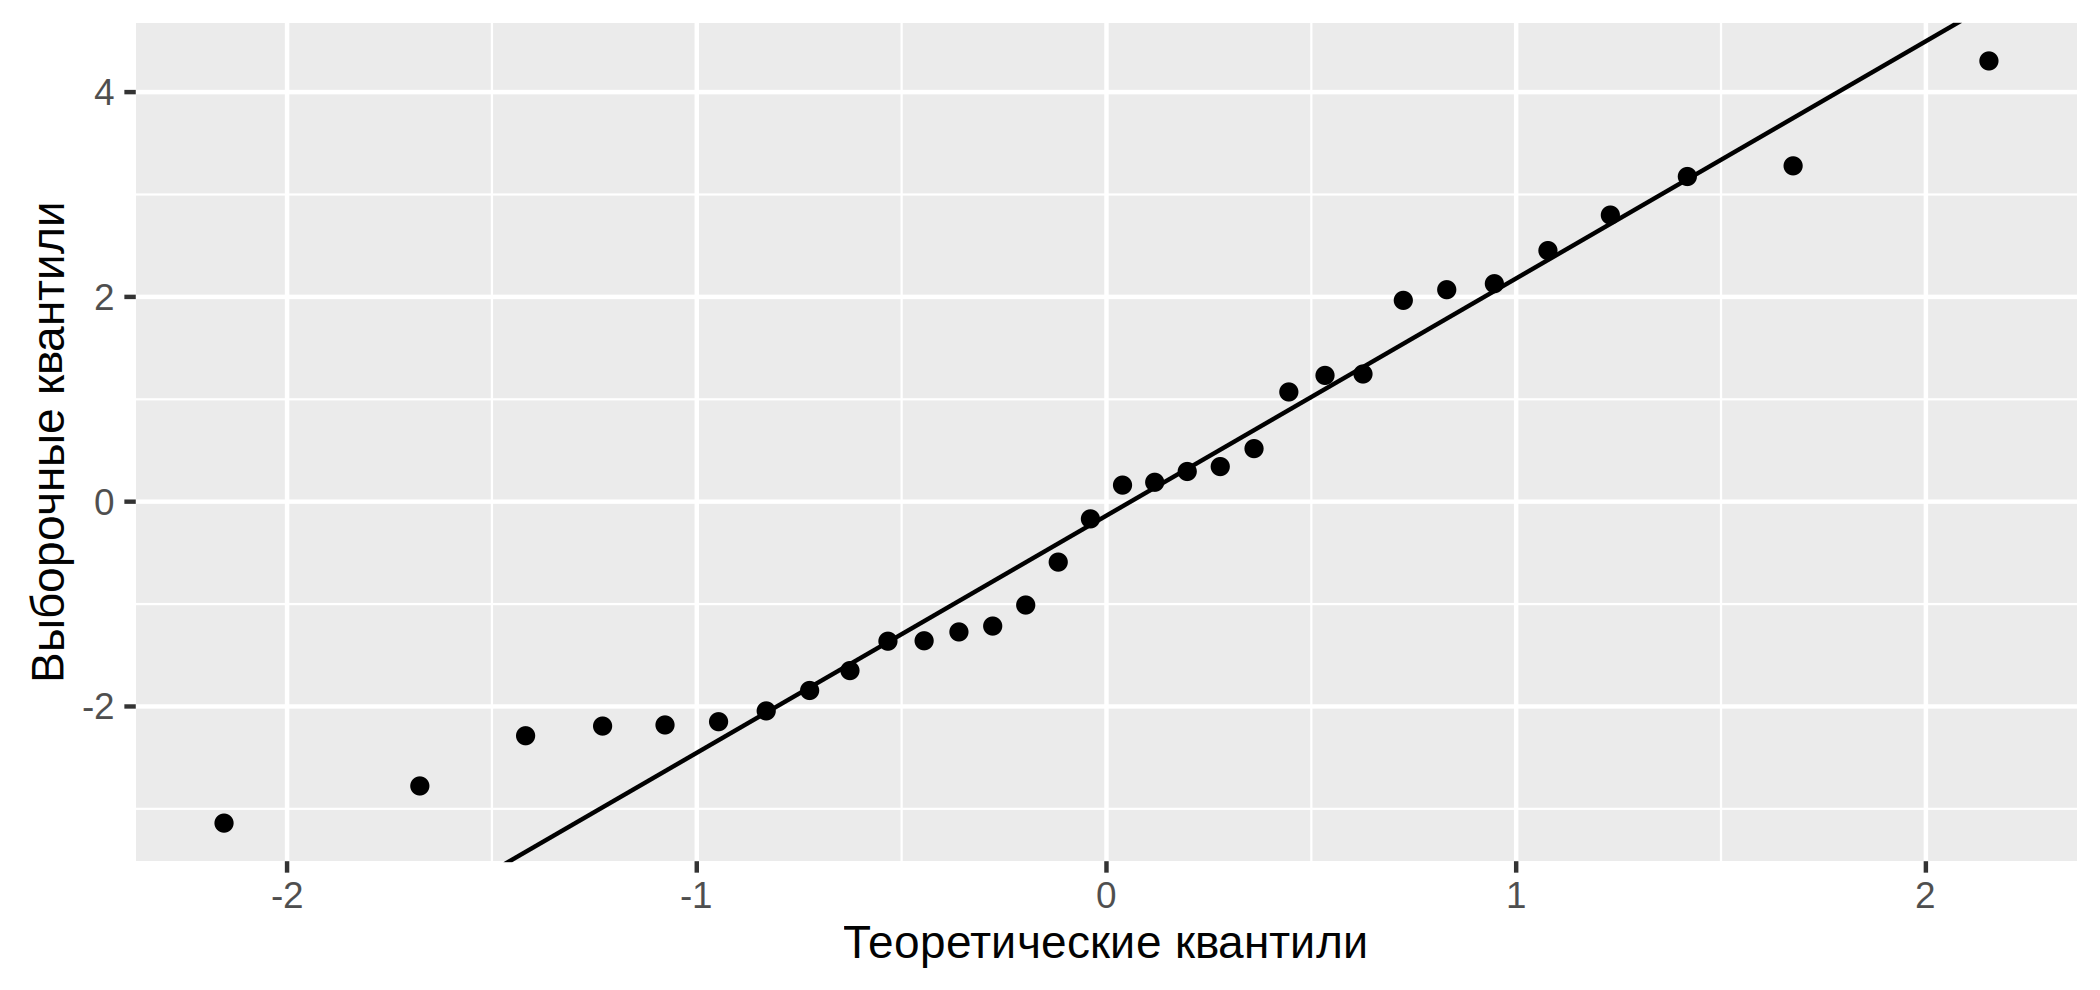
\includegraphics[width=1\linewidth]{../figures/residual/quantile.png}}
\caption{График квантилей для остатков}
\label{img:resid_qqnorm}
\end{figure}
На рисунке \ref{img:resid_qqnorm} можно заметить, что присутствуют отклонения относительно нормального распределения. Наиболее явный из них --- нижний хвост. Остальные --- небольшие скачки по ходу линии нормального распределения. Проверим с помощью критерия Шапиро-Уилка, можно ли считать полученные остатки нормально распределёнными. Из полученных в \textbf{R} результатов, статистика Шапиро--Уилка $ W = \test{residual}{shapiro}{statistic} $. Вероятность ошибки $ p = \test{residual}{shapiro}{p-value} > 0.05 $, а значит нулевая гипотеза не отвергается. Следовательно опровергнуть предположение о нормальности на основе данного теста нельзя.

Проверим критерий $ \chi^2 $ Пирсона. Из полученных в \textbf{R} результатов, статистика $\chi^2$ Пирсона $ P = \test{residual}{pearson}{statistic}$. Вероятность ошибки $ p = \test{residual}{pearson}{p-value} > 0.05 $, а значит нулевая гипотеза не отвергается.% TODO: Устаревшие вычисления // Реализовать в R // можно удалить

Построим график автокорреляционной функции для определения наличия взаимосвязей в ряде остатков (рисунок \ref{img:resid_acf}). На графике пунктирные линии разграничивают значимые и не значимые корреляции: значения, выходящие за линии, являются значимыми \cite[с.376]{Teetor2011RCook}.
\begin{figure}[ht]
	\center{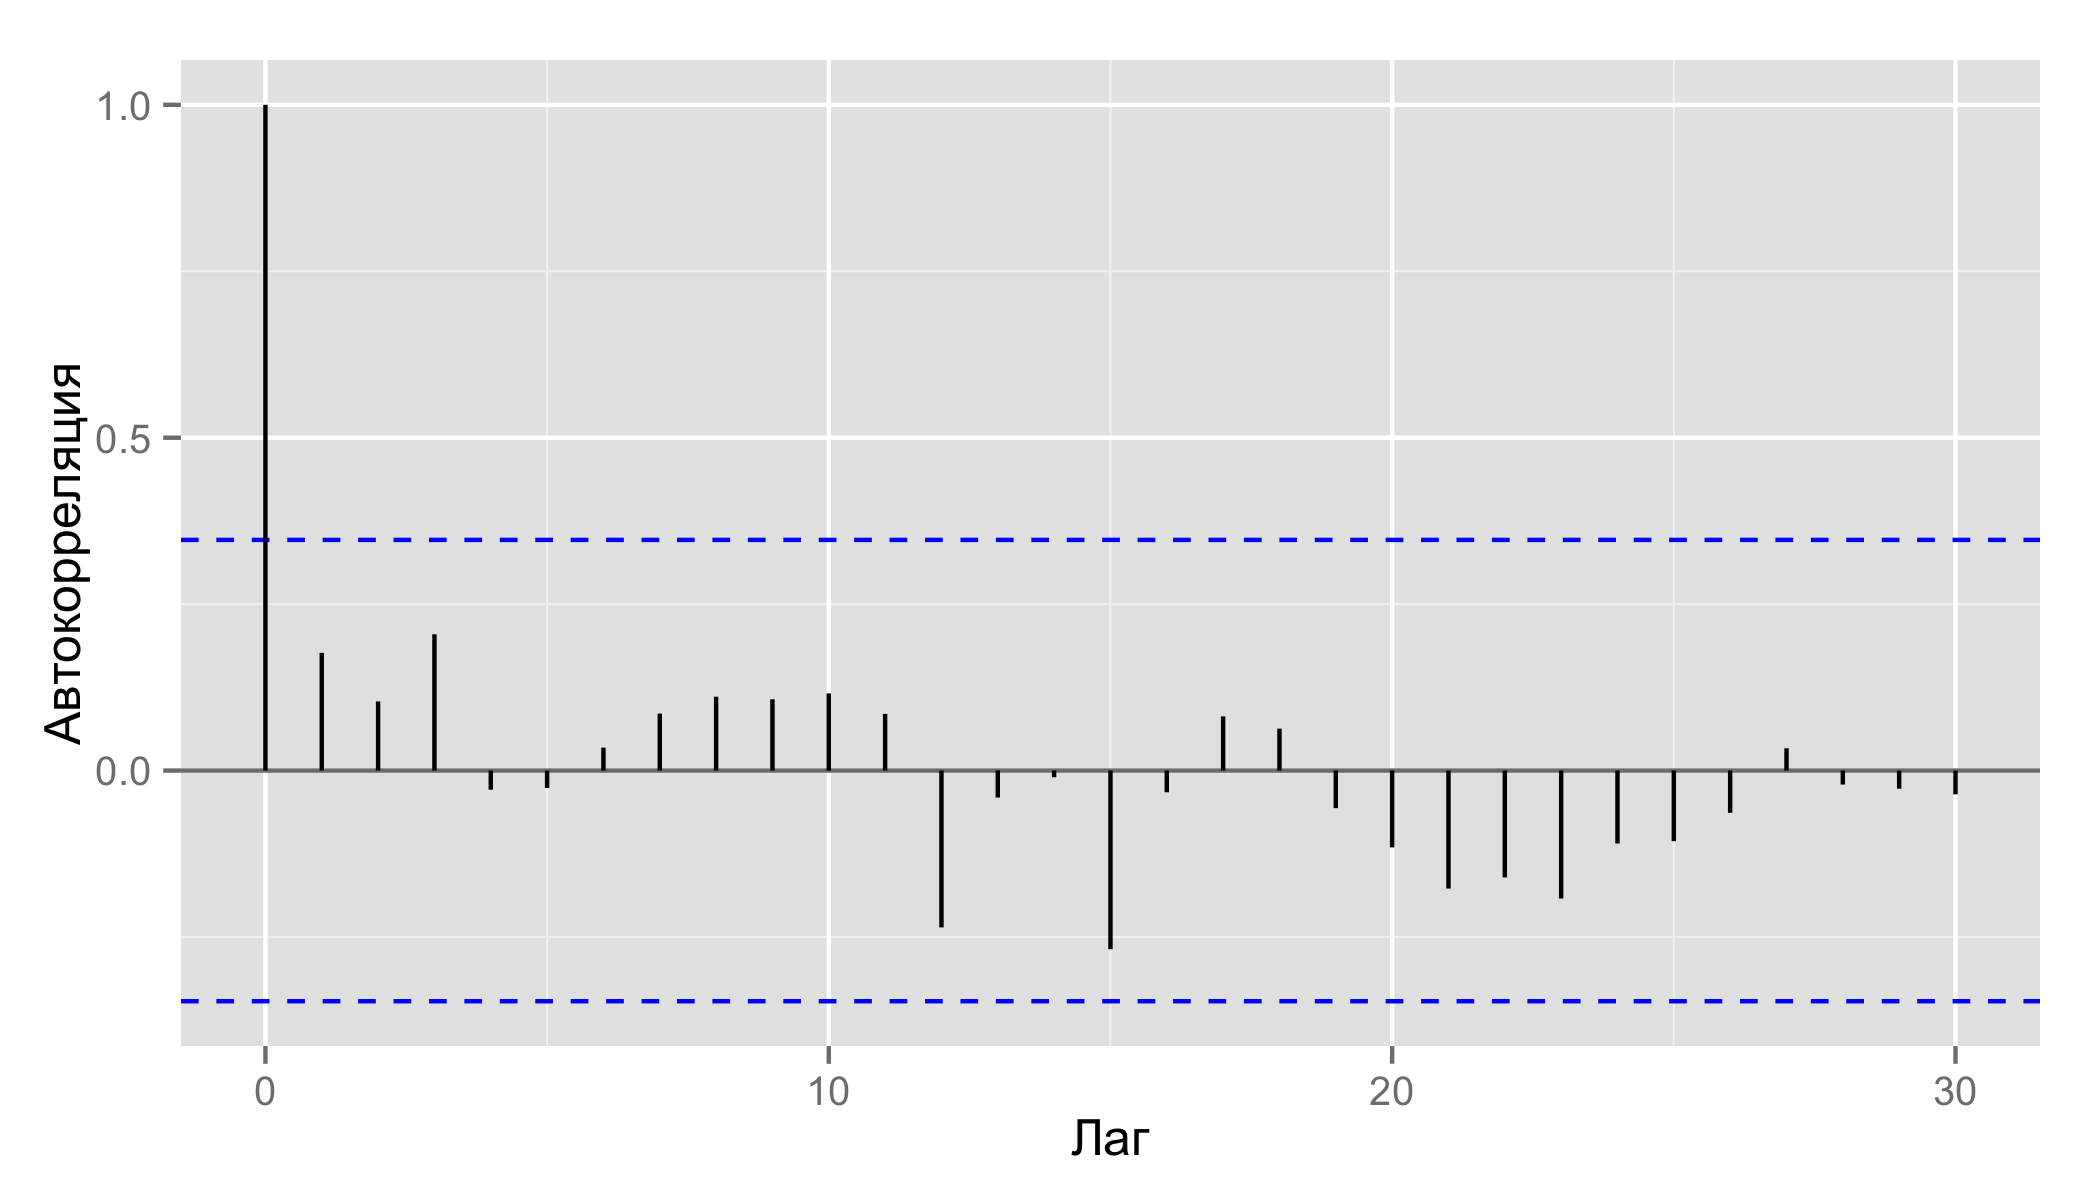
\includegraphics[width=1\linewidth]{../figures/residual/acf.png}}
\caption{График автокорреляционной функции}
\label{img:resid_acf}
\end{figure}% TODO: ТУТ ПЛОХОВАТО НАПИСАНО // немного поменял, но не уверен
На представленном графике автокорреляционной функции все значения не выходят за интервал, обозначенный пунктирными линиями. Это означает, что в представленной автокорреляционной функции нету значимых автокорреляций. Проверим это замечание с помощью теста Льюнга-Бокса \cite[с.377-378]{Teetor2011RCook}. Данный тест позволяет проверить наличие автокорреляций в исследуемых данных. Используя возможности пакета \textbf{R} получили значения: статистика Льюнга--Бокса $ X^2 = \test{residual}{ljung-box}{statistic} $ и вероятность ошибки $ p = \test{residual}{ljung-box}{p-value} > 0.05$ --- это говорит о том, что тест не выявил значимых автокорреляций.

На рисунке \ref{img:resid_acf} также можно заметить некоторое затухание значений автокорреляций с увеличением лага. На основе этого можно сделать предположение о стационарности. Для проверки этого предположения воспользуемся расширенным тестом Дики--Фуллера(ADF) \cite{Dickey1979Distribution}. Из результатов проверки теста, статистика Дики-Фуллера $ DF = \test{residual}{stationarity}{statistic} $, вероятность ошибки $ p = \test{residual}{stationarity}{p-value} < 0.05 $. Следовательно, при уровне значимости $ \alpha = 0.05 $ необходимо принять альтернативную гипотезу о стационарности.
% TODO: надо подумать. p-value для обрезанного ряда оказался не вери-гуд // ПОДОГНАТЬ

% TODO: нужно проапдейтить вывод -- он плохой // проапдейтил // независимые ~ нет автокорелляций
Таким образом в результате анализа детерминированными методами выделены две составляющие исходной модели данных: тренд и нерегулярная составляющая. В ходе регрессионного анализа было показано, что модель, основанная на тренде, не позволяет воспроизвести поведение исходного временного ряда. То есть нерегулярная составляющая $ \varepsilon(t) $ является существенной и отвечает за это поведение. Для того, чтобы определить возможность её дальнейшего исследования проведен анализ остатков, в процессе которого показаны близость распределения к нормальному (с некоторыми отклонениями) и стационарность, при этом не выявлено значимых автокорреляций. Таким образом, это позволяет перейти к построению модели другими, современными статистическими методами интерполяции. Улучшение модели будет происходить за счёт суперпозиции модели, полученной на данном этапе, и найденной модели нерегулярной составляющей.

% subsubsection analysis_residuals (end)

% section determenistic (end)

\section{Геостатистический подход} % (fold)
\label{sec:geostatistic}

Традиционные детерминированные модели интерполяции, широко используемые в задачах прогнозирования, в большинстве случаев на практике не позволяют в полной мере решить ту или иную задачу. В наиболее благоприятных вариантах исследований они позволяют оценивать значения в точках, в которых измерения не проводились. В свою очередь, анализ этих данных и его результаты в значительной мере зависят как от качества так и от количества исходных данных. И именно такие результаты были получена в результате проведенного в предыдущем разделе исследования. А также сделан вывод о необходимости использования современных методов исследования.

В современных исследованиях аналогичного класса задач усилился интерес к геостатистическим моделям интерполяции, что подтверждается работами \cite{GeoStCompar1987, GeoStCompar1998}. Современная геостатистика --- это широкий спектр статистических моделей и инструментов для анализа, обработки и представления пространственно-распределенной информации.

В частности, широкое распространение получили модели из семейства \textit{кригинга}. Преимущество данного семейства перед детерминированными методами в том, что они позволяют получить наилучшую в статистическом смысле оценку  --- несмещенную оценку с минимальной дисперсией, при этом оценка кригинга сопровождается оценкой ошибки интерполяции в каждой точке. Полученная ошибка позволяет охарактеризовать неопределенность интерполяционной оценки данных при помощи доверительных интервалов.

% TODO: НУ, ТУТ ВСЕ ПЛОХО

\subsection{Вариограммный анализ. Кригинг.} % (fold)
\label{sec:_variogram}
% Тут постановка задачи про то, что использую остатки и т.п.
В последующем исследовании в качестве объекта анализа будем использовать нерегулярную составляющую $ \varepsilon(t) $. Поэтому исследуемой выборкой будем считать остатки, полученные на этапе регрессионного анализа и представленные в приложении \ref{c:app_results} в таблице \ref{table:residuals}. Проведённый анализ остатков выявил стационарность, независимость и близость к нормальному распределению. Из условий накладываемых на вариограмму (ссылку на теорию, свою и не очень), следует возможность её применения.

Центральная идея геостатистики состоит в использовании знаний о корреляции экспериментальных данных для построения оценок и интерполяций. \textit{Вариограмма} является ключевым инструментом для оценки степени корреляции, имеющейся в исследуемых данных, и для ее моделирования. Модель вариограммы является функцией, определяющей зависимость изменения исследуемой величины от расстояния. Следовательно, интерполяционная модель, основанная на такой корреляционной функции, будет отражать реальные явления, которые лежат в основе данных измерений. Всевозможные пары точек могут быть рассортированы по классам в соответствии с разностью их координат
\begin{equation*}
	h = x_i - x_j, \quad i, j = \overline{1,n}, \quad i \neq j,
\end{equation*}
называемой \textit{лагом}. Для близких точек разность значений функции в них обычно меньше и растет с увеличением расстояния между точками. Вычислив среднее значение квадратов разностей для каждого значения лага $h$, можно получить дискретную функцию, называемую \textit{экспериментальной вариограммой}. Вариограмма обычно характеризуется двумя параметрами: \textit{рангом} и \textit{порогом}. Порог характеризует предельное значение вариограммы, на некотором расстоянии, называемом рангом, за которым последующие значения вариограммы становятся некоррелированными.
%Эффект самородков характеризуется разрывом вариограммы около нуля.

Для оценки поведения данных при увеличении лага построим диаграмму взаимного разброса пар точек (\textit{h-scatterplot}), разделённых расстоянием $ h $. Эта диаграмма позволяет проверить наличие корреляции в исследуемых данных как качественно, так и количественно \cite{saveliev2012}. Построенная диаграмма изображена на рисунке \ref{img:hscat} в приложении \ref{c:graphs}. Следует отметить, что в классическом случае присутствия зависимости, поведение должно быть следующим: на графиках, соответствующим начальным лагам, должна присутствовать сильная корреляция, и с увеличением лага корреляция уменьшается. Это объясняется тем, что чем ближе находятся данными тем выше зависимость между ними и наоборот. В рассматриваемом случае такого не наблюдается. Напротив, на первом же лаге отсутствует корреляция, при этом можно наблюдать, что на некоторых лагах присутствует корреляция, на некоторых нет. Такое поведение свойственно так называемым беспороговым моделям вариограммы. Другими словами, моделям, в которых отсутствует ранг. Одной из таких моделей является линейная, с которой некоторые исследователи советуют начинать подбор модели. Аргументируется это тем, что она является простейшей. Поведение диаграммы в рассматриваемом случае, вообще говоря, вполне обосновано спецификой исследуемых данных: рассматривается температура воды за один определённых месяц в течение нескольких лет. Ко всему прочему, это подтверждается результатами проведённого ранее анализа остатков, в котором мы выяснили, что ошибка распределение ряда остатков является близким к нормальному и значения некоррелируемы и независимы.

В некоторых источниках советуют при построении вариограммы учитывать параметр максимального расстояния, для которого вычисляется вариограмма, а также приводят рекомендацию по его подбору. Поэтому первоначальным параметром было выбрано значение, рассчитанное по такой рекомендации: $ 2n / 3 = 21 $ \cite{cressie2011statistics}.

Экспериментальной вариограммой по сути является некоторая оценка вариограммы. Существует несколько известных оценок, каждая из которых имеет свои достоинства и недостатки. Для данного исследования были выбраны наиболее распространённые: оценка Матерона \eqref{eq:var_estimation}, введённая ранее в главе 2, и оценка Кресси-Хокинса \cite{cressie1993statistics, dutter}:
\begin{equation*}
	2 \tilde{\gamma}(h) = \frac{1}{n - h} (\sum_{t = 1}^{n - h} | X(t + h) - X(t) |^{\frac{1}{2}} )^4 / (0.457 + \frac{0.494}{n - h} + \frac{0.045}{(n - h)^2}), \quad h = \overline{0, n - 1},
\end{equation*}
для сравнения полученных результатов.

Как уже было сказано ранее, случайный процесс $ \varepsilon{t} $ удовлетворяет всем нужным свойствам !!!!! для вариограммного анализа. Сначала проведём исследования с помощью оценки Матерона, затем сравним полученные результаты с
оценкой Кресси-Хокинса.

Построенная вариограмма отображена на рисунке \ref{img:classical-variogram} в приложении \ref{c:graphs}. На представленном рисунке можно заметить, что на промежутке $[0;1]$ не происходит роста значений вариограммы. Наоборот, наблюдается разрыв: первое значение находится значительно выше $0$. При этом вариограмма не сильно выходит за пределы дисперсии переменной, которая равна $4.07$. Более того, первые значения уже достигло порога. Что говорит о том, что вариограмма на первых значениях выходит на предельное значение, и последующие значения некоррелированы. Это, на самом деле, согласуется с исследуемыми исходными данными, так как при анализе остатков было выявлено отстутсвие автокорреляций, и спецификой самих данных: наблюдение за каждый год, вообще говоря, не зависит от предшедствующего.

На основе этого делаем вывод о наличии эффекта самородков и делаем первоначальное предположение о равенстве порога $3.9$.

На основе экспериментальной вариограммы построим модель вариограммы для дальнейшего использования на этапе кригинга. Моделью вариограммы может служить не каждая функция, а только та, для которой выполнено условие положительной определенности. Положительная определенность модели вариограммы гарантирует, что уравнения кригинга, построенные с использованием данной модели, имеют единственное устойчивое решение. Поэтому при моделировании используются только те функции, для которых положительная определенность установлена, а также их взвешенные линейные комбинации с неотрицательными весами, которые тоже будут являться положительно определенными. Модель вариограммы строится как линейная комбинация подходящих базисных моделей \cite{saveliev2012}.

Для построения моделей вариограммы существует два подхода: вручную, т.е. визуально с ручным подбором параметров, и автоматическим подбором параметров с помощью специальных методов. И на практике построение модели вариограммы представляет собой итеративный процесс, на каждом шаге которого следует наилучшим образом подобрать параметры очередного модельного приближения. В различной литературе рекомендуется строить моделей вручную, так как исследователь лучше знает специфику данных, чем различные методы оценивания. Попробуем построить модель вариограммы визуально.

% Тут где-то нужно ввести эффект самородков с описанием, что он делает

Ранее было отмечено присутствие эффекта самородков. Другой, часто встречающейся моделью, является сферическая:
\begin{equation}
	\gamma(\vert h \vert) = c Sph_a(\vert h \vert) = \left\{
 \begin{array}{l l}
   c(1.5 \vert h \vert / a - 0.5(\vert h \vert / a)^3) &, \vert h \vert \le a, \\
   \\
   c &,	 \vert h \vert > a.
 \end{array} \right.
\end{equation}

Возьмём эту модель в качестве базовой с помощью функции \textit{vgm}, в качестве начального параметра возьмём порог, указанный ранее: $3.9$. Далее воспользуемся функцией \textit{fit.variogram} для подбора более точных значений указанной модели. Таким образом окончательная модель:
% latex table generated in R 3.1.3 by xtable 1.7-4 package
% Sat May 30 20:33:43 2015
\begin{table}[H]
\centering
\begin{tabular}{rlrr}
  \hline
 & Модель & Порог & Ранг \\ 
  \hline
1 & Nug & 0.00 & 0.00 \\ 
  2 & Per & 4.10 & 0.90 \\ 
   \hline
\end{tabular}
\caption{Модель вариограммы} 
\label{table:manual_model}
\end{table}

И график полученной модели на рисунке \ref{img:var-models} (пунктиром). На графике можно проследить все указанные ранее особенности: эффект самородков и порог.
\begin{figure}[ht]
	\center{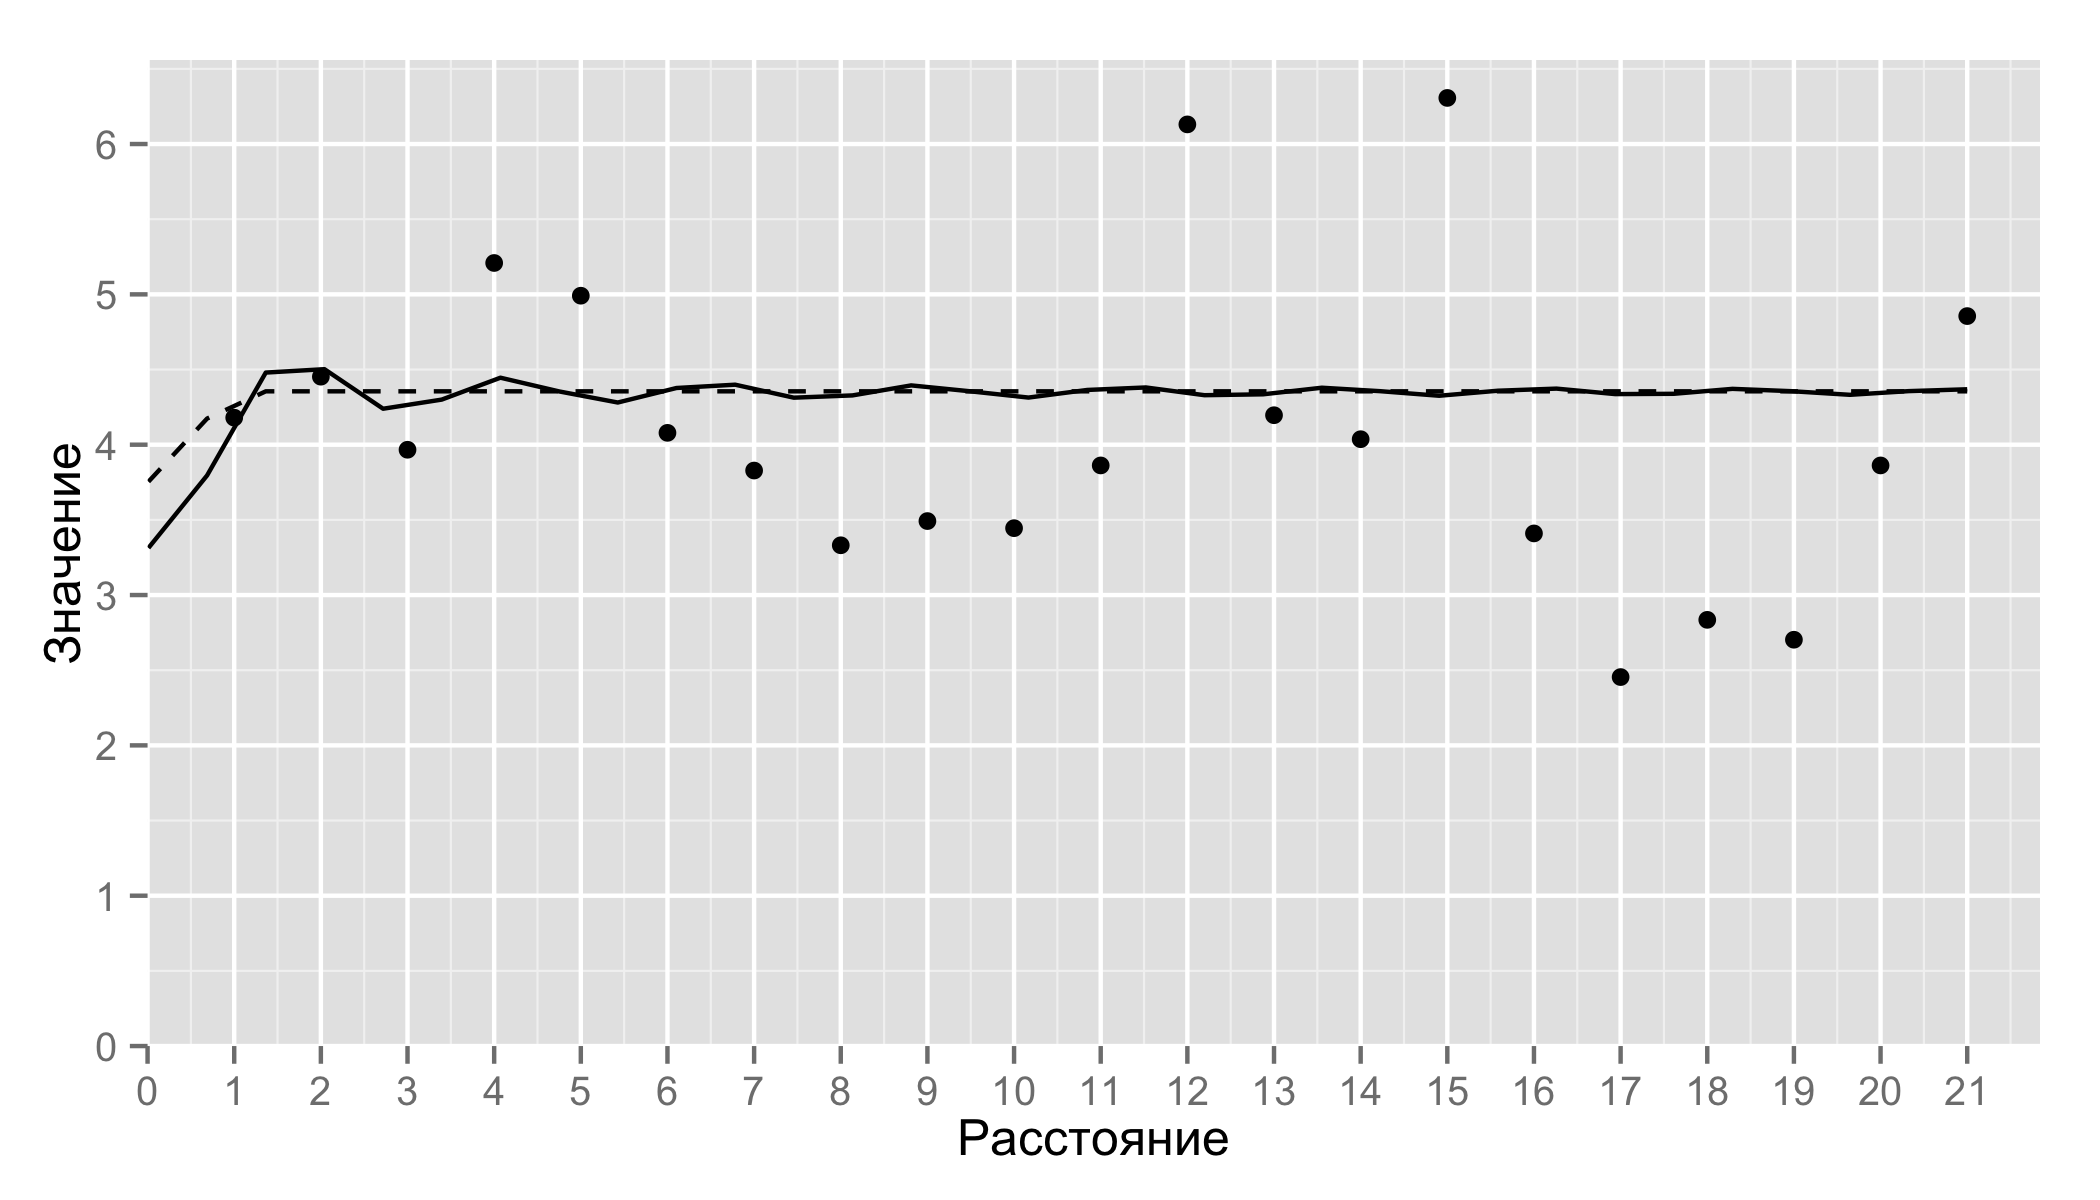
\includegraphics[width=1\linewidth]{../figures/variogram/models-comparison.png}}
\caption{Классические модели вариограммы}
\label{img:var-models}
\end{figure}

Задача геостатистики --- оценить значения изучаемой пространственной переменной в произвольных точках области исследования на основе анализа ее значений, измеренных в ограниченном числе выборочных точек. По построенной модели вычислим оценки при помощи ординарного кригинга, реализованного функцией \textit{krige}. Вычисленные значения отображены в таблице \ref{table:manual-prediction} в приложении \ref{c:app_results}. Оценку отклонения от истинных значений выразим с помощью среднеквадратической ошибки \textit{(MSE)}. В данном случае $ MSE = \characteristic{variogram}{manual-mse} $. Полученные значения оказались идентичными значению тренда, следовательно прогноз почти не изменился. Это говорит о том, что построенная модель не смогла уловить поведение исходных данных. По этой причине был использован второй вариант построения модели --- c автоматическим подбором параметров.

Для построения модели вариограммы была реализована возможность автоматического подбора модели на основе функции \textit{fit.variogram}. Суть этого подхода заключается в следующем: при заданных начальных условиях (эффект самородков, ранг, порог), для всех возможных базисных моделей подгонялись их параметры, для этих моделей вычислялись сумма квадратов ошибок, и на основе этого показателя выбиралась наиболее эффективная модель. Код программы представлен в листинге \ref{lst:main}.

На рисунке \textbf{[DELETED]} сплошной линией и в приложении \ref{c:graphs} на рисунке \ref{img:manual-variogram} показан результат выполнения представленной ранее функции. Таким образом, наилучшей моделью вариограммы, построенной по классической оценке, стала линейная комбинация двух: эффект самородков с параметром $ \characteristic{variogram}{classical-nug} $ и модель с эффектом дыр (\textit{Hole}) с параметрами: порог --- $ \characteristic{variogram}{classical-psill} $, ранг --- $ \characteristic{variogram}{classical-range} $ изображенная в приложении \ref{c:graphs} на рисунке \ref{img:classical-variogram}.

Методом простого кригинга в этом случае были построены прогнозные значения, отображенные в таблице \ref{table:classical-prediction}.
% latex table generated in R 3.1.2 by xtable 1.7-4 package
% Fri May 15 14:21:08 2015
\begin{table}[ht]
\centering
\begin{tabular}{rrrrr}
  \hline
 & Год & Наблюдение & Прогноз & Тренд \\ 
  \hline
1 & 2007 & 19.400 & 21.714 & 21.578 \\ 
  2 & 2008 & 21.800 & 21.578 & 21.687 \\ 
  3 & 2009 & 21.900 & 21.881 & 21.797 \\ 
  4 & 2010 & 24.300 & 21.876 & 21.906 \\ 
  5 & 2011 & 22.800 & 22.013 & 22.016 \\ 
  6 & 2012 & 20.200 & 22.171 & 22.126 \\ 
   \hline
\end{tabular}
\caption{Прогноз (классическая оценка)} 
\label{table:classical-prediction}
\end{table}

Полученные значения отличаются от предыдущих, в них появилось некоторое поведение. Но в данном случае $ MSE = \characteristic{variogram}{classical-mse} $, что хуже предыдущего значения, а значит, прогноз ухудшился.
Попробуем улучшить результат с помощью робастной оценки Кресси.

Модель вариограммы, представленная на рисунке \ref{img:robust-variogram} в приложении \ref{c:graphs}, является также линейной комбинацией двух базисных моделей: эффекта самородков с параметром $ \characteristic{variogram}{robust-nug} $ и волновая модель с параметрами: $ \characteristic{variogram}{robust-psill} $, $ \characteristic{variogram}{robust-range} $. Заметим, что эмпирическая вариограмма, построенная по робастной оценке, отличается от соотвествующей вариограмм, построенных по классической оценке. Появилось заметное поведение вариограммы, в отличие от предыдущей, где значения концентрировались около дисперсии выборки.

Результаты применения кригинга показали прогнозные значения, указанные в \ref{table:robust-prediction}.
% latex table generated in R 3.1.2 by xtable 1.7-4 package
% Fri May 15 14:21:09 2015
\begin{table}[ht]
\centering
\begin{tabular}{rrrrr}
  \hline
 & Год & Наблюдение & Прогноз & Тренд \\ 
  \hline
1 & 2007 & 19.400 & 21.458 & 21.578 \\ 
  2 & 2008 & 21.800 & 21.748 & 21.687 \\ 
  3 & 2009 & 21.900 & 21.940 & 21.797 \\ 
  4 & 2010 & 24.300 & 22.027 & 21.906 \\ 
  5 & 2011 & 22.800 & 22.055 & 22.016 \\ 
  6 & 2012 & 20.200 & 22.089 & 22.126 \\ 
   \hline
\end{tabular}
\caption{Прогноз (робастная оценка)} 
\label{table:robust-prediction}
\end{table}

Среднеквадратическая ошибка $ MSE = \characteristic{variogram}{robust-mse} $, таким образом это значение близко к значению, полученному вручную. Таким образом, использование робастной оценки улучшило результат применения кригинга.

\begin{figure}[ht]
	\center{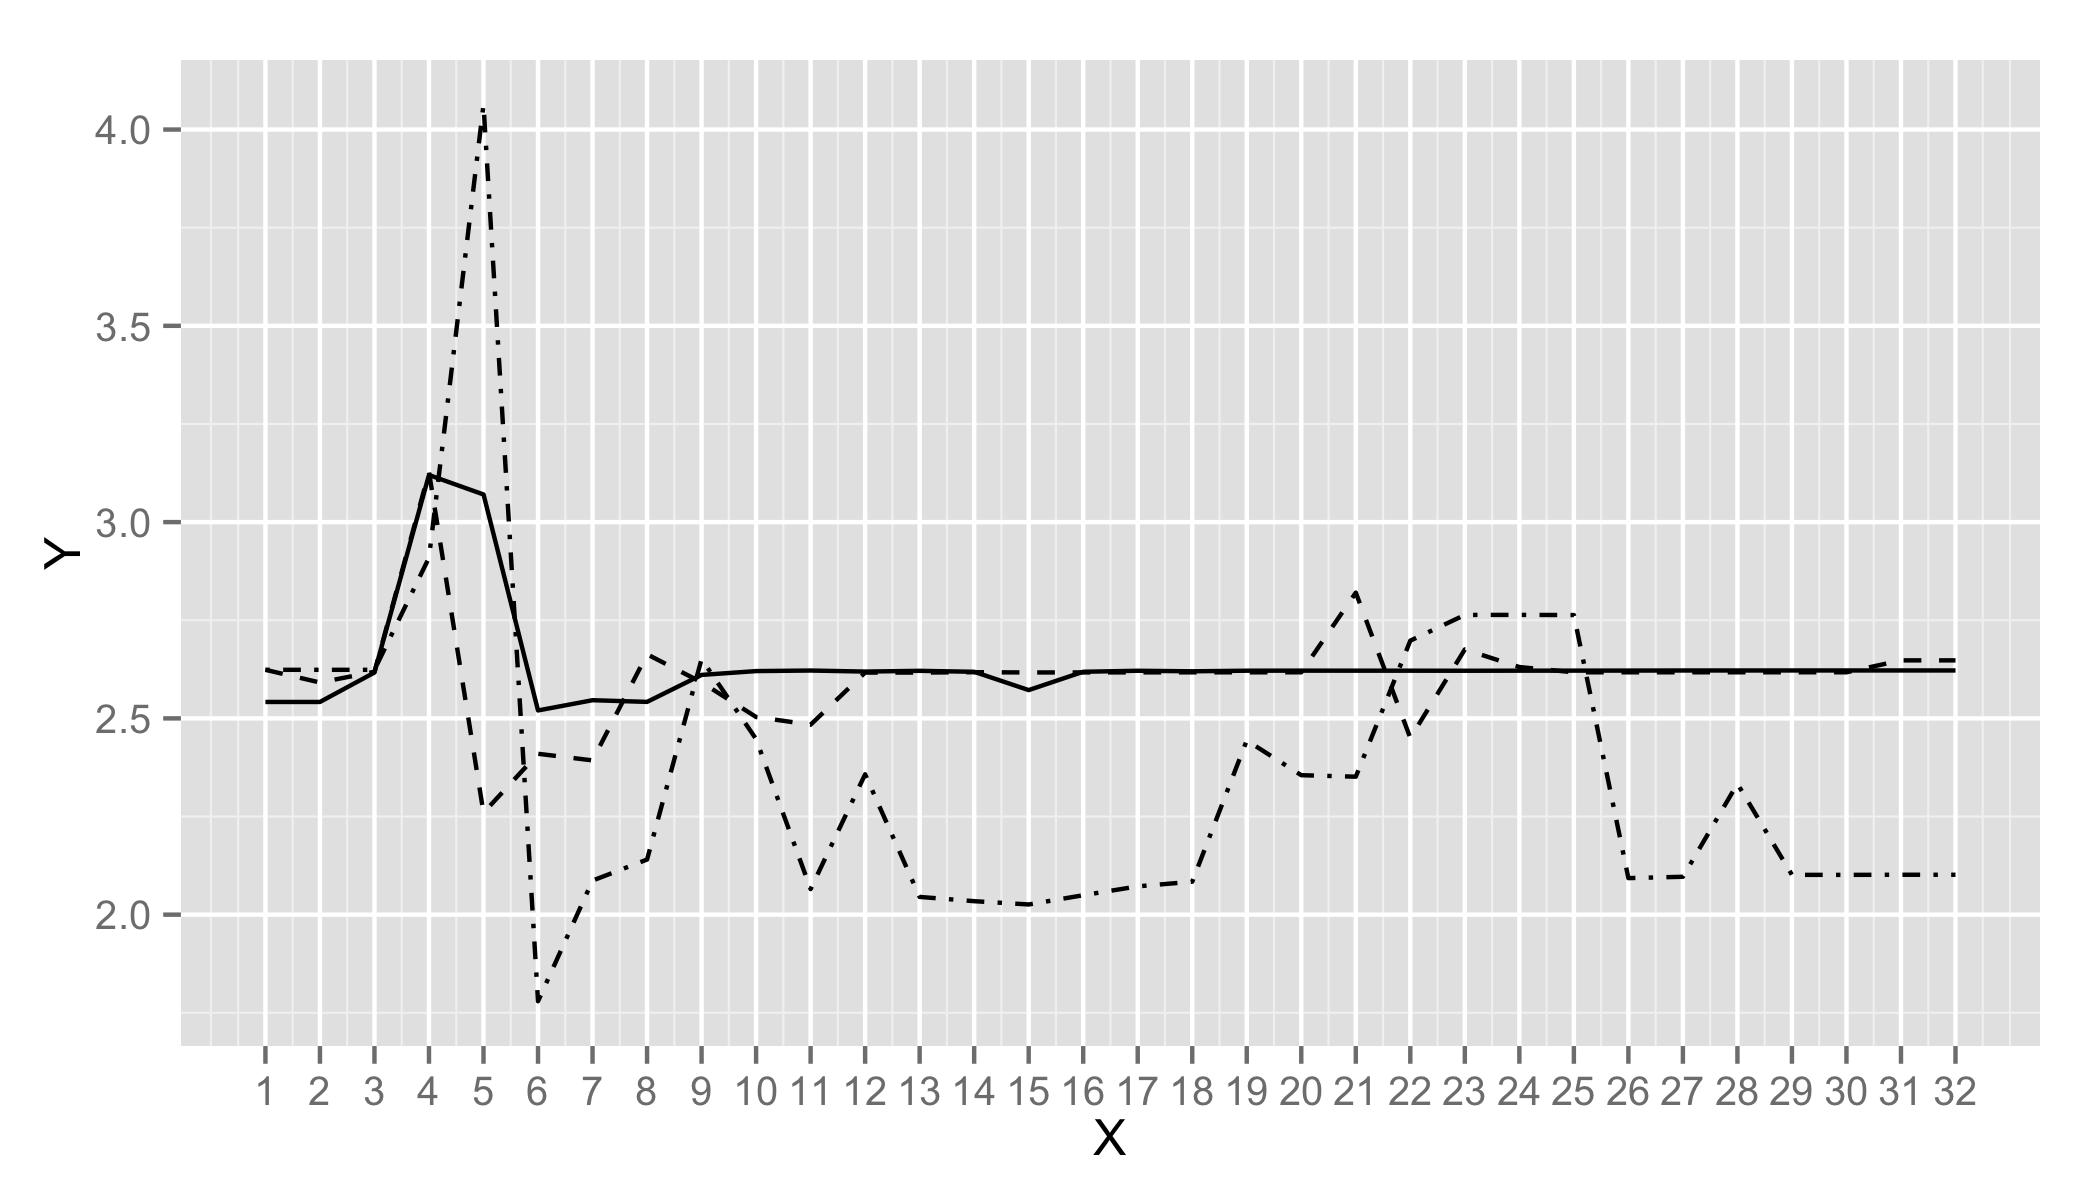
\includegraphics[width=1\linewidth]{../figures/variogram/parameter-comparison.png}}
\caption{Зависимость ошибки от максимального расстояния}
\label{img:check-dep}
\end{figure}

Исследуем теперь поведение прогнозных значений, полученных с помощью кригинга, при различных параметрах максимального расстояния вариограммы. В качестве оценки качества полученного прогноза возьмем среднеквадратическую ошибку. Чем меньше ошибка --- тем лучше прогноз. Для этих целей реализована функция \textit{ComparePredictionParameters}. Результат её работы на рисунке \ref{img:check-dep}. На этом графике отчетливо видно, что робастная оценка (пунктир-точка), в отличие от классической (пунктир) и модели, построенной вручную (сплошная), в большинстве случаев даёт более точные прогнозы. И наилучший при максимальном расстоянии равным $6$. С этим параметром, наилучший прогноз составляют значения кригинга из \ref{table:robust-best-prediction}.
% latex table generated in R 3.1.3 by xtable 1.7-4 package
% Tue May 19 03:07:19 2015
\begin{table}[ht]
\centering
\begin{tabular}{rrrrr}
  \hline
 & Год & Наблюдение & Прогноз & Тренд \\ 
  \hline
1 & 2007 & 19.400 & 21.154 & 21.578 \\ 
  2 & 2008 & 21.800 & 21.626 & 21.687 \\ 
  3 & 2009 & 21.900 & 22.046 & 21.797 \\ 
  4 & 2010 & 24.300 & 22.302 & 21.906 \\ 
  5 & 2011 & 22.800 & 22.365 & 22.016 \\ 
  6 & 2012 & 20.200 & 22.290 & 22.126 \\ 
   \hline
\end{tabular}
\caption{Наилучший прогноз (робастная оценка)} 
\label{table:robust-best-prediction}
\end{table}

Среднеквадратическая ошибка оказалась равной $ MSE = \characteristic{variogram}{robust-best-mse} $. Что действительно является лучшим из полученных показателем.

Сравнительный анализ полученного прогноза представлен на графике \ref{img:robust-best-cross-prediction} в приложении \ref{c:graphs}.

Таким образом в результате вариограммного анализа были исследованы различные модели вариограмм, оценки, проведены два подхода по вычислению. В результате кригинга построена наилучшая модель прогнозных значений. Которая в свою очередь имеет погрешность в пределах стандартного отклонения. Следовательно данная модель является хорошим вариантом для построения прогнозных значений.

% subsection _variogram (end)

% section geostatistic (end)